%%%%%%%%%%%%%%%%%%%%%%%%%%%%%%%%%%%%%%%%%
% Stylish Article
% LaTeX Template
% Version 2.1 (1/10/15)
%
% This template has been downloaded from:
% http://www.LaTeXTemplates.com
%
% Original author:
% Mathias Legrand (legrand.mathias@gmail.com) 
% With extensive modifications by:
% Vel (vel@latextemplates.com)
% Final ACS by:
% Juan Barbosa
% License:
% CC BY-NC-SA 3.0 (http://creativecommons.org/licenses/by-nc-sa/3.0/)
%
%%%%%%%%%%%%%%%%%%%%%%%%%%%%%%%%%%%%%%%%%
\documentclass[fleqn,10pt]{SelfArx}
%\usepackage[superscript]{cite}
\usepackage{wrapfig}
%----------------------------------------------------------------------------------------
%	ARTICLE INFORMATION
%----------------------------------------------------------------------------------------

\JournalInfo{Laboratorio Avanzado, No. 1, 03/03/2017} % Journal information
\Archive{ }

\PaperTitle{S\'intesis de Dilantin un antiepileptico a partir de benzaldehido} %
%\Keywords{Keyword1 --- Keyword2 --- Keyword3} % Keywords - if you don't want any simply remove all the text between the curly brackets
%\newcommand{\keywordname}{Keywords} % Defines the keywords heading name

%----------------------------------------------------------------------------------------
%	ABSTRACT
%----------------------------------------------------------------------------------------

\Abstract{
\begin{wrapfigure}{r}{0.45\textwidth}
\centering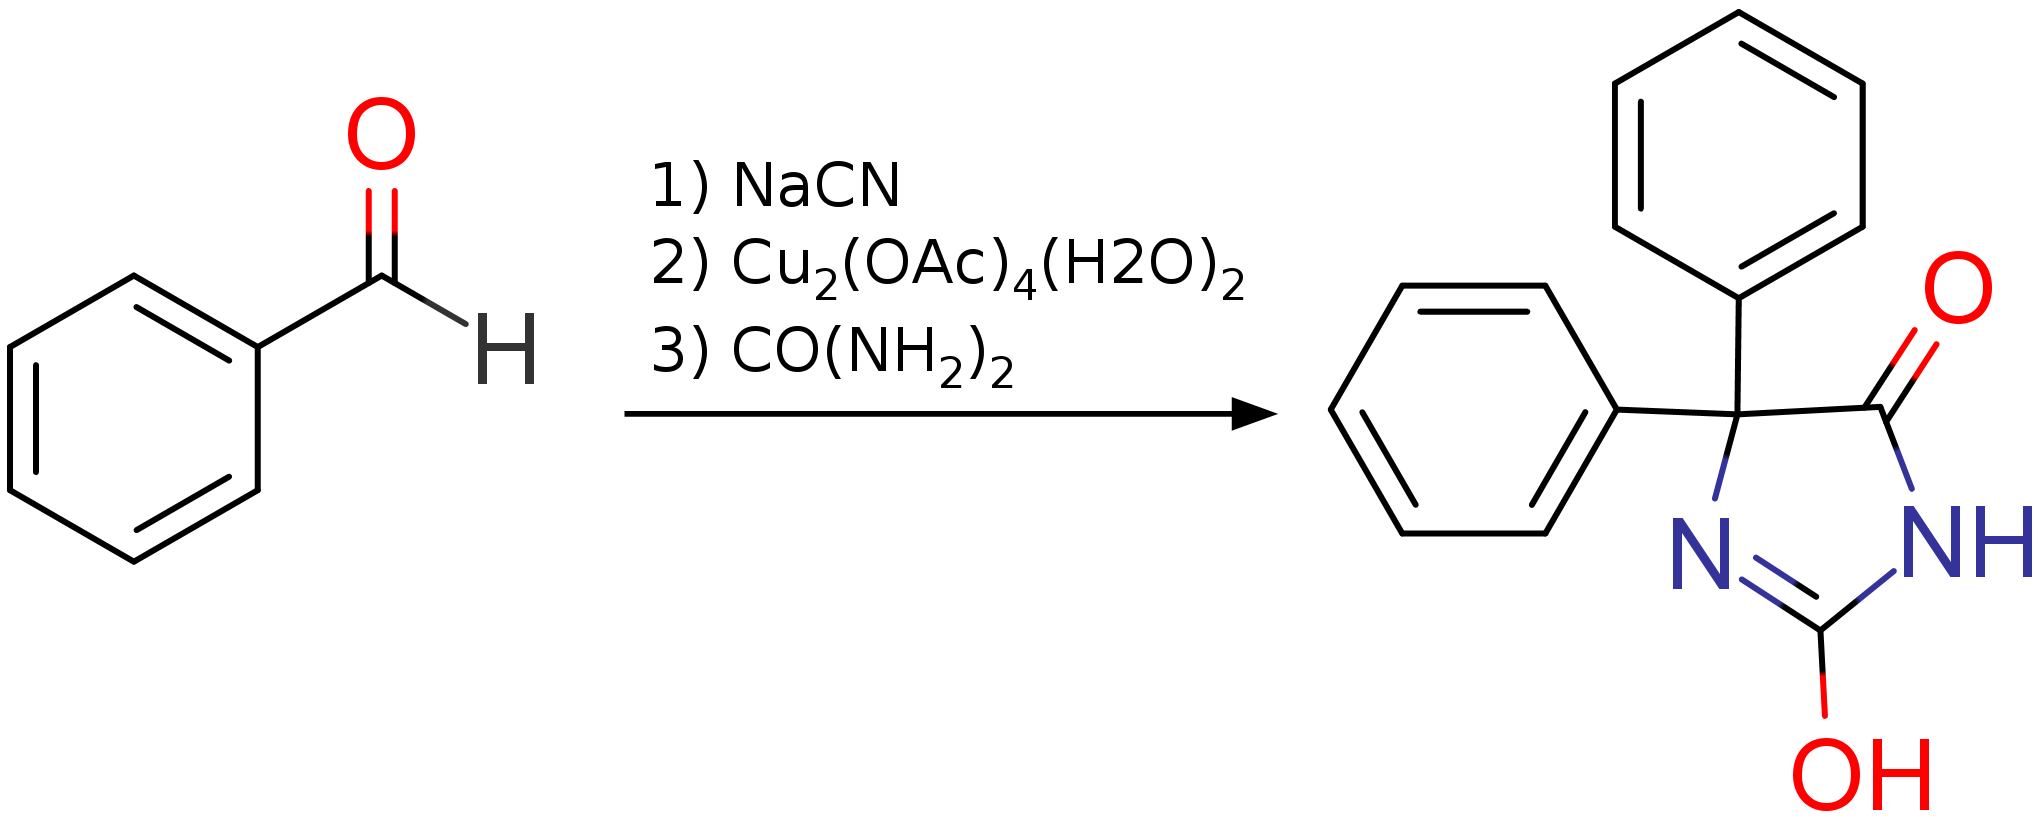
\includegraphics[scale=1]{structures/overall.png}
\end{wrapfigure}
La s\'intesis de la 5,5-difenilimidazolidina-2,4-diona (\textit{Dilantin}) se realiza en 3 etapas a partir del benzaldeh\'ido. La primera corresponde con una condensaci\'on benzo\'inica, la segunda es la oxidaci\'on de la benzo\'ina y finalmente se lleva a cabo la condensaci\'on con \'urea y un rearreglo benz\'ilico para dar origen al compuesto hidanto\'inico. Las \'ultimas dos etapas son realizadas con dos metodolog\'ias distintas, la primera novedosa y la segunda cl\'asica, usando cerca de la mitad de la benzo\'ina sintentizada en cada una. Los rendimientos obtenidos por las dos rutas son 11\% y 15\% correspondientemente. Siendo la ruta cl\'asica m\'as apropiada en t\'erminos de rendimiento y pureza, sin embargo la m\'as demandante en tiempo.
}

%----------------------------------------------------------------------------------------

\begin{document}

\flushbottom % Makes all text pages the same height

\maketitle % Print the title and abstract box

%\tableofcontents % Print the contents section

\thispagestyle{empty} % Removes page numbering from the first page



%----------------------------------------------------------------------------------------
%	ARTICLE CONTENTS
%----------------------------------------------------------------------------------------

\section*{Introducci\'on} % The \section*{} command stops section numbering
Las hidantoínas son un grupo de moléculas que comparten el mismo anillo heterocíclico, denominado hidantoína (2,4-imidazolidinadiona) \cite{m2015}\cite{kroschwitz2007}. Dicho anillo se caracteriza por ser plano y bastante rígido \cite{m2015}, además de raramente encontrarse en productos naturales \cite{kroschwitz2007}. Estas moléculas son sólidos cristalinos con altos puntos de fusión.
\begin{scheme}[h]
	\centering
	\caption{Anillo de hidanto\'ina.}
	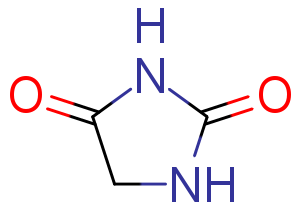
\includegraphics[width=0.3\linewidth]{structures/hydantoin.png}
\end{scheme}

Este tipo de moléculas tiene una amplia gama de aplicaciones, siendo su uso farmacéutico uno de los más difundidos. Entre sus aplicaciones médicas está el uso como antiepiléptico, agente antiarrítmico, agente antitumoral, bactericida y fungicida \cite{safari2010}\cite{ildiz2012}\cite{hayward1983}. Sin embargo también se encuentran en diferentes productos cosméticos, sanitarios, agrícolas e industriales \cite{kroschwitz2007}. En química su importancia reside en su uso como agentes para cloración o bromación \cite{m2015}, reactivos analíticos \cite{kroschwitz2007} y la preparación de $\alpha$-aminacidos por medio de la hidrólisis básica de estos compuestos \cite{m2015}. La primera síntesis de la 5,5-difenilimidazolidina-2,4-diona (Dilantin) fue en 1908 por el químico alemán Heinrich Biltz, el cual trabajo con varias hindantoínas \cite{hayward1983}\cite{aicardi2007}. Esta molécula se utiliza para el tratamiento de la epilepsia. Su funcionamiento se basa amortiguar la actividad cerebral descontrolada que se presenta en el momento de las convulsiones. Esto se realiza mediante la reducción de la conductancia eléctrica entre las neuronas por medio de la estabilización del voltaje de los canales de sodio \cite{asif2015}. Desde su obtención en 1908, se han propuesto distintos métodos de síntesis entre los cuales se encuentran: en fase sólida, one-pot, en pasos múltiples y asistida por ultrasonido \cite{safari2010}. La ruta sintética usada comercialmente es el tratamiento de benzofenona con cianuro de potasio acuoso y carbonato de amonio, reacci\'on que recibe el nombre de Bucherer-Bergs \cite{hayward1983}\cite{li2013}\cite{kadam2007}. 
\begin{scheme}[h]
	\centering
	\caption{S\'intesis comercial del Dilant\'in, reacci\'on de Bucherer-Bergs \cite{li2013}.}
	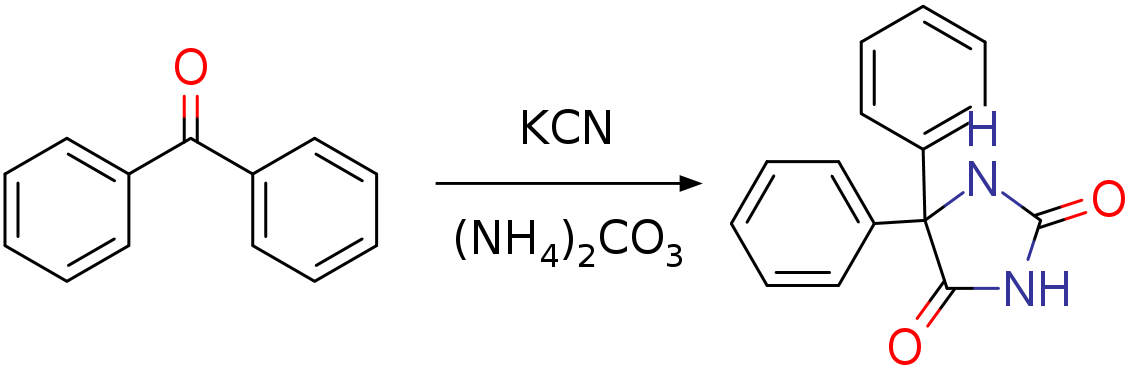
\includegraphics[width=0.8\linewidth]{structures/bucherer.png}
\end{scheme}

El procedimiento experimental usado en la presente s\'intesis fue realizado en tres pasos divididos en la s\'intesis de la benzo\'ina, la oxidaci\'on de la misma para obtener benzil, y finalmente la condensaci\'on con \'urea y el rearreglo benz\'ilico. La obtenci\'on de la benzo\'ina se realiz\'o con una condensaci\'on benzo\'inica en presencia de cianuro de sodio. La oxidaci\'on de la misma se llev\'o a cabo usando dos m\'etodos distintos, el primero propuesto por Depreux \cite{depreux1988} en donde el cobre act\'ua como catalizador de la reacci\'on, y el segundo donde se usa \'acido n\'itrico. El \'ultimo paso de la reacci\'on usa los mismos reactivos para ambos m\'etodos, con la diferencia que el primero es asistido por ultrasonido y el segundo se lleva a cabo en reflujo \cite{safari2010}.
\begin{scheme}[h]
	\centering
	\caption{S\'intesis del Dilantin con las dos rutas seguidas en el laboratorio.}
	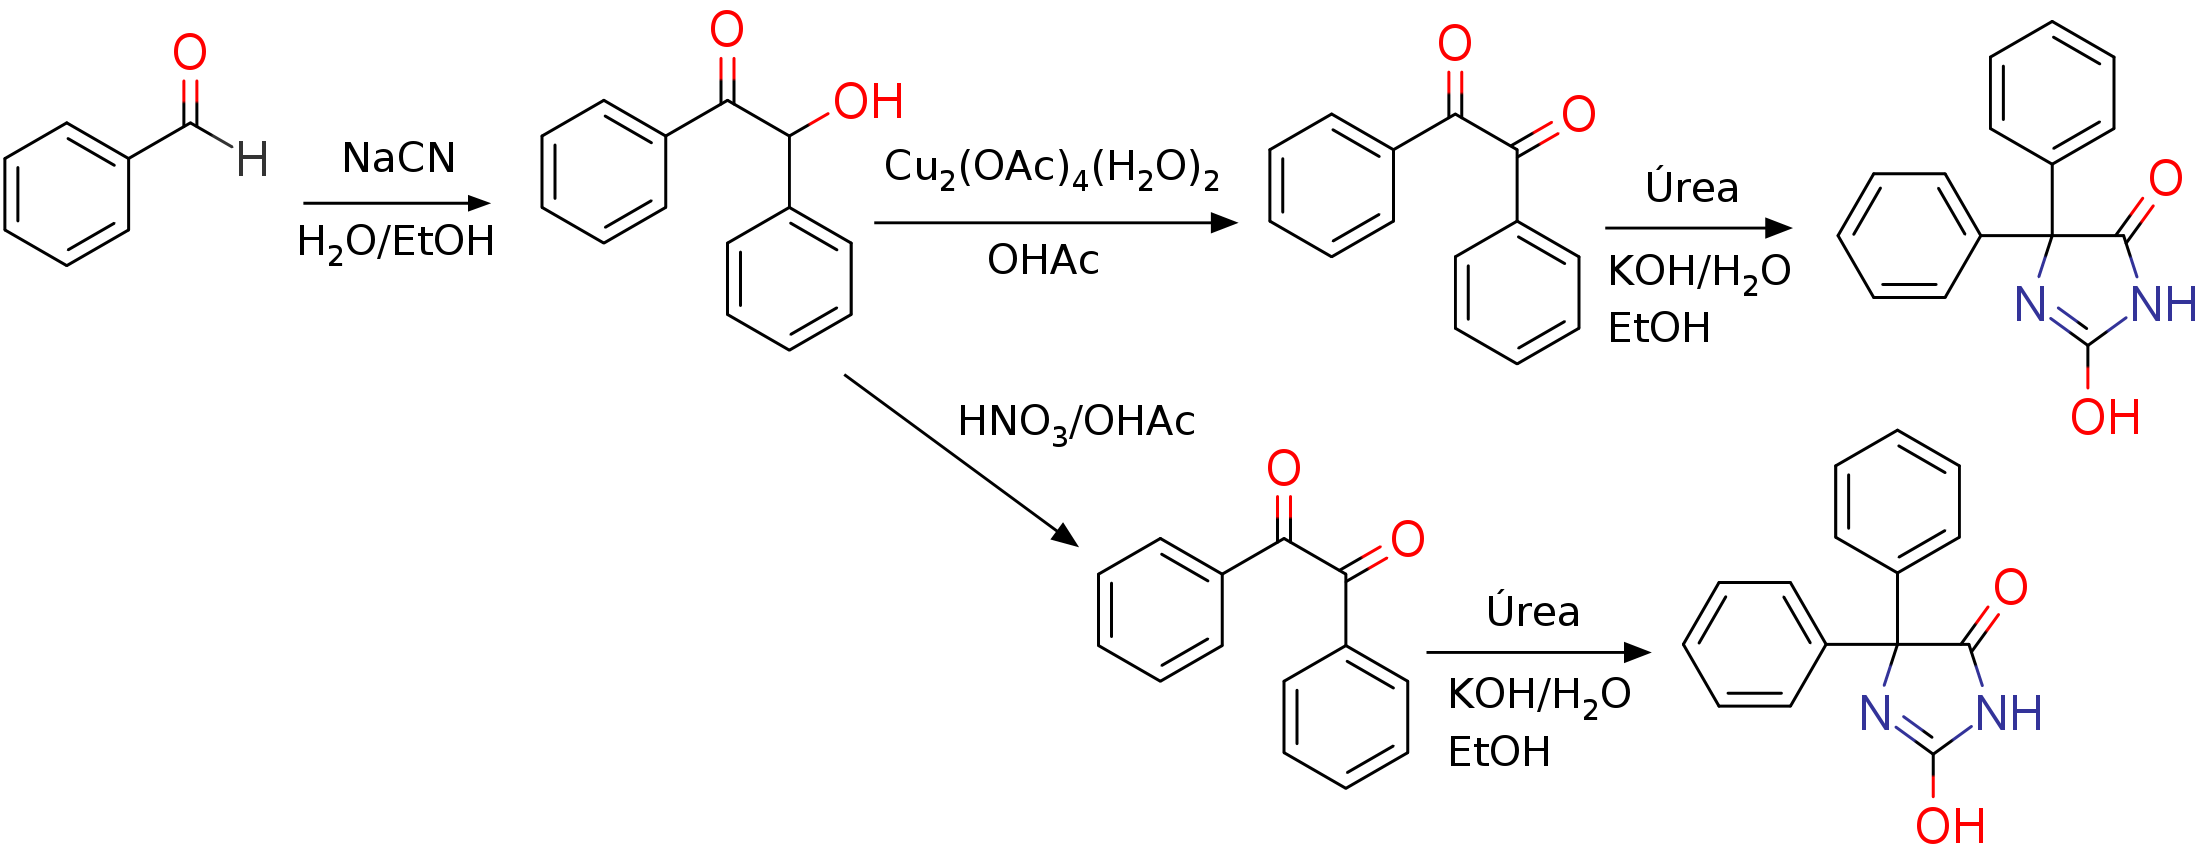
\includegraphics[width=\linewidth]{structures/complete.png}
\end{scheme}

%------------------------------------------------

\newpage
\section{Resultados y Discusi\'on}
Los rendimientos obtenidos para las distintas etapas y m\'etodos se muestran en el \autoref{tb: resultados}. El rendimiento neto usando los m\'etodos alternativos es de 11 \% y la s\'intesis cl\'asica present\'o un rendimiento total de 15 \%. Si bien la diferencia parece ser poco significativa esto se debe al bajo rendimiendo de la condensaci\'on benz\'ilica, puesto que si analiza el rendimiento a partir de la benzo\'ina se tiene: 50 \% y 70 \% correspondientemente para cada l\'inea, alternativa y cl\'asica.
\begin{table}[h]
	\centering
	\caption{Rendimientos obtenidos en el laboratorio.}
	\label{tb: resultados}
	\begin{tabular}{ccc}
		\hline
		\textbf{Reacci\'on} & \textbf{Metodo} & \textbf{Rendimiento \%} \\
		\hline
		Condensaci\'on & \'unico & 22 \\
		Oxidaci\'on & acetato & 78 \\
		Oxidaci\'on & \'acido & 87 \\
		Rearreglo & ultrasonido & 63 \\
		Rearreglo & reflujo & 71 \\
		\hline
	\end{tabular}
\end{table}

La primera etapa de la síntesis de Dilantin consiste en la obtención de benzoina, para ello se hizo reaccionar benzaldehído con cianuro. El rendimiento de la reacción obtenido fue del 22\%. El bajo rendimiento de la reacción se justifica con un mal proceso de recristalización donde se perdió la mayoría del producto. El problema con la recristalización fue que había mucho producto y por ello fue necesario utilizar grandes cantidades de etanol caliente, por lo que al enfriar la solución esta no se saturó y no precipitó todo la benzoina que se formó. Además, por limitaciones de tiempo no fue posible evaporar el etanol del filtrado y volver a enfriar para de este modo recuperar el producto de forma cuantitativa. El producto obtenido fue caracterizado por medio de $^1$H-RMN. En este se ven varios picos a campo bajo debido a la presencia de grupos extractores de carga como el oxígeno, además el campo inducido por el campo electromagnético sobre el anillo aromático desprotege aún más los hidrógenos adyacentes. La señal en 0 ppm corresponde al TMS y las señales entre 1 y 4 ppm corresponden a trazas de etanol que se encontraban dentro del tubo de RMN. El singlete en 4.56 ppm corresponde al hidrógeno del hidroxilo (a), mientras que el singlete en 5.95 ppm corresponde al H del carbono unido al hidroxilo (b). El multiplete entre 7.2 y 7.55 ppm corresponde a los hidrógenos aromáticos del fenil adyacente al alcohol y los hidrógenos \textit{-meta} del fenil adyacente al carbonilo (c). El triplete en 7.5 ppm corresponde al hidrógeno del fenil en posición \textit{-para} al carbonilo (d) y se separa del multiplete de aromáticos debido a que por resonancia el carbono al que está unido adquiere una carga parcial negativa. Por último, el doblete en 7.9 ppm (e) corresponde a los hidrógenos orto al carbonilo, estos están más desplazados que todos los otros hidrógenos aromáticos tanto por efecto mesomérico como inductivo. A partir del espectro se evidencia que la benzoina obtenida está pura.
\begin{scheme}[h]
	\centering
	\caption{Asignaci\'on de protones para la benzo\'ina.}
	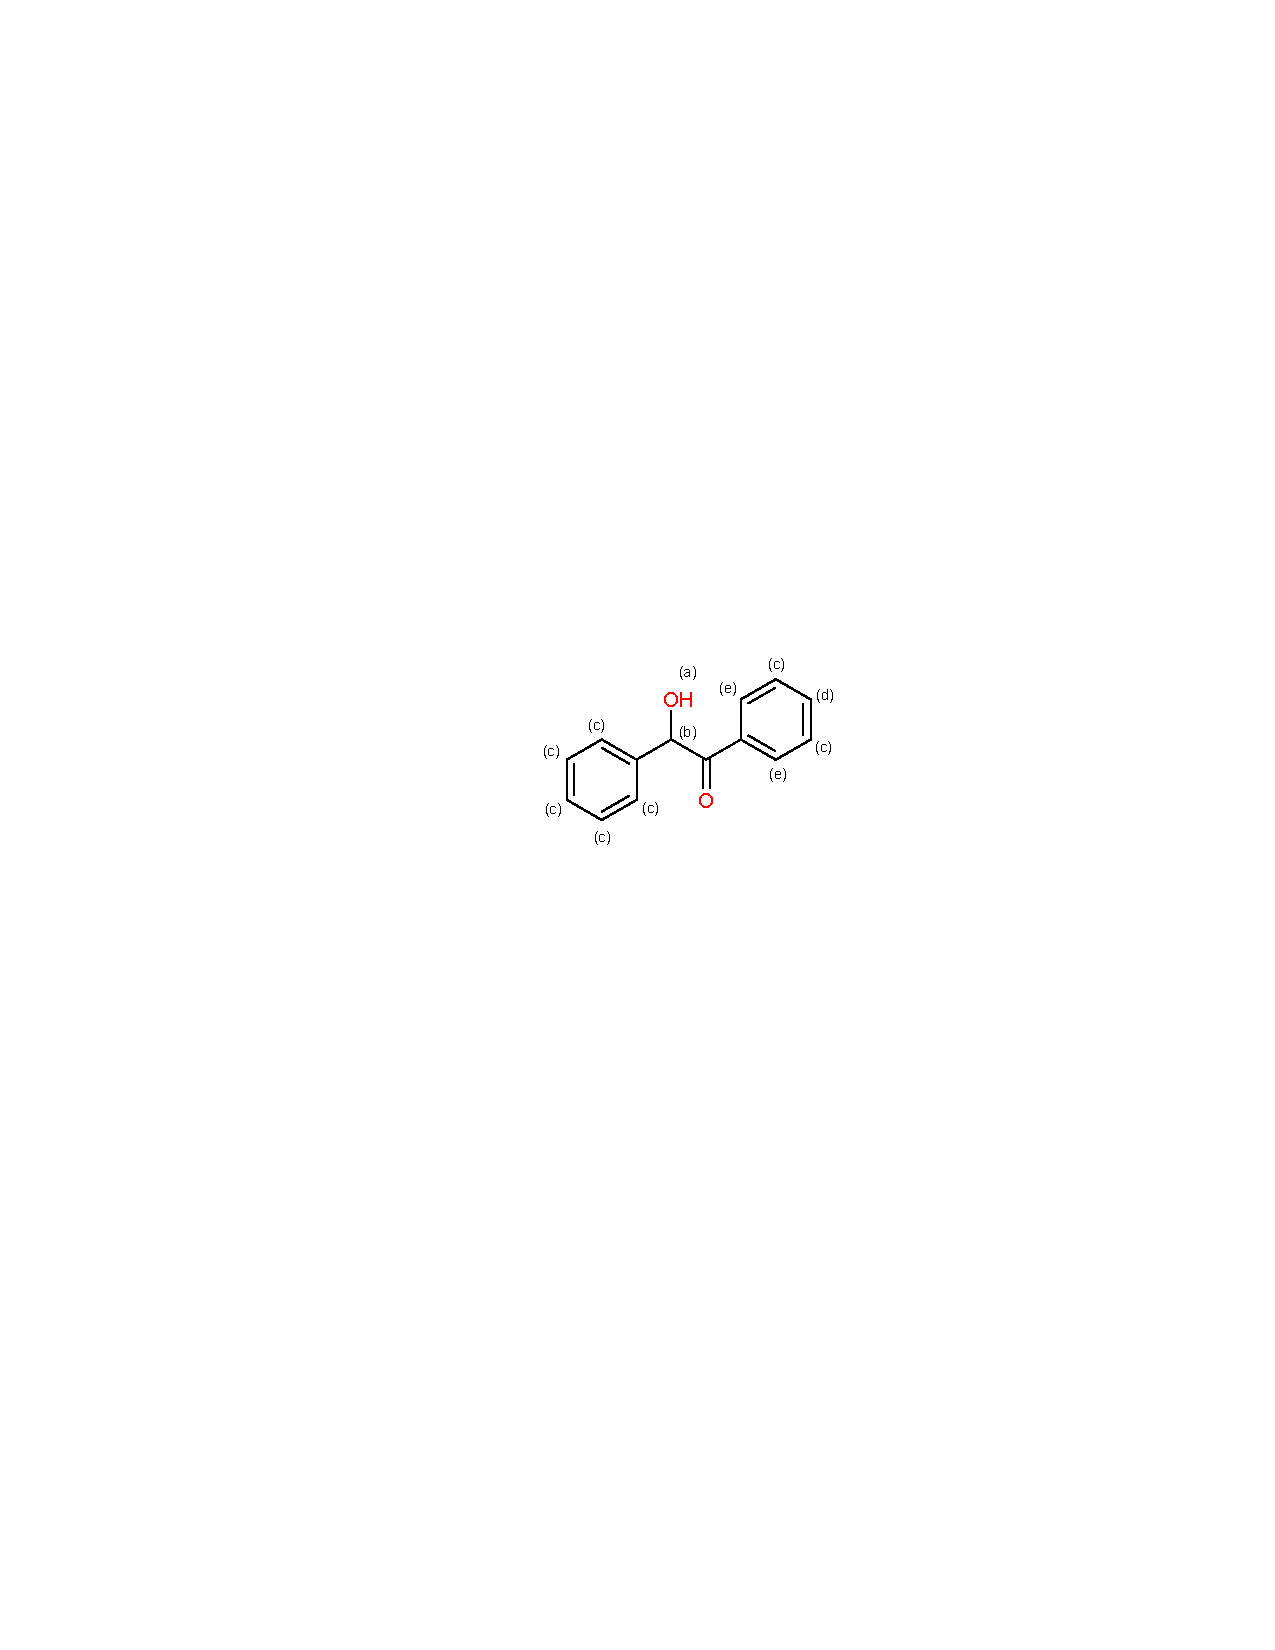
\includegraphics[width=0.6\linewidth]{structures/picos_benzoina.pdf}
\end{scheme}


El mecanismo de la reacción se fundamenta en tres propiedades fundamentales del cianuro: su gran nucleofilicidad, su habilidad para estabilizar cargas negativas en posiciones $\alpha$ a este y sus propiedades como buen grupo saliente \cite{cyanideioncatalyzedbenzoincondensation2014}. La reacción comienza con el ataque nucleofílico del cianuro al carbonilo del benzaldehído \textbf{(1)}, formando un intermediario tetraédrico que se protona con una molécula de agua del medio \textbf{(2)}, dando lugar a la cianohidrina \textbf{(3)}. El protón de la cianohidrina es relativamente ácido debido al efecto inductivo del hidroxilo y el nitrilo, por lo que puede ser retirado por una molécula de agua formando una carga negativa sobre este carbono. Dicha carga es estabilizada por resonancia con el anillo aromático o también con el nitrilo, en este caso dando lugar a un aminoceteno \textbf{(4)}. El par electrónico del nitrógeno puede volver a regenerar el nitrilo, causando un ataque nucleofílico sobre el carbono del benzaldehído formando el compuesto \textbf{(5)}. Este último se protona y da lugar a un diol \textbf{(6)}. Una molécula del medio puede deprotonar el hidroxilo geminal al nitrilo y debido a que este es un buen grupo saliente se da la eliminación \textbf{(7)} de cianuro para formar benzoina \textbf{(8)}.
\begin{scheme}[h]
	\centering
	\caption{Mecanismo de condensaci\'on benzo\'inica.}
	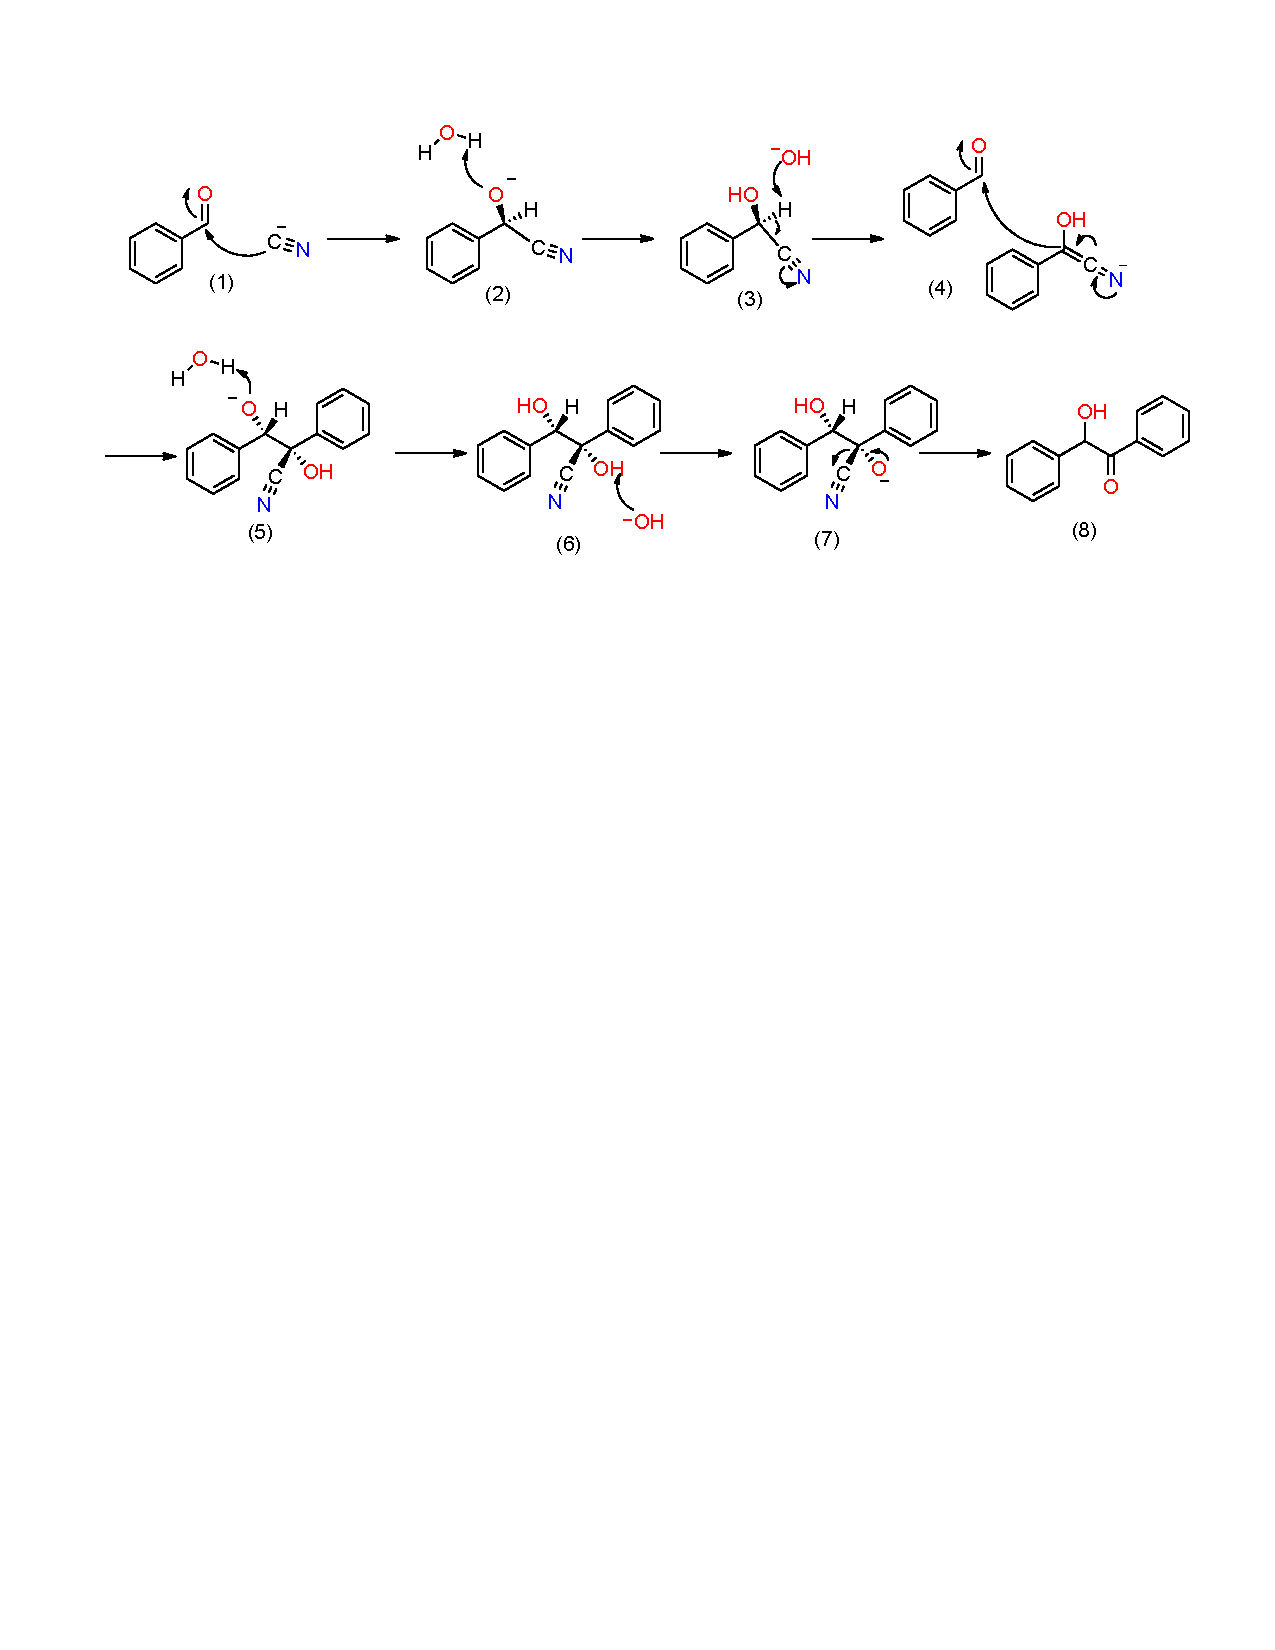
\includegraphics[width=\linewidth]{structures/mecanismo_benzoina.pdf}
\end{scheme}

Se creía que el paso determinante de la reacción era la formación del enlace C-C, sin embargo estudios computacionales indican que existen otros estados de transición que también afectan de forma significativa la velocidad de reacción \cite{yamabe2009}. En orden decreciente de energía se tiene: formación enlace C-C \textbf{(4)} (+22.12 kcal/mol), eliminación de cianuro \textbf{(7)} (+20.96 kcal/mol) y remoción del protón ácido \textbf{(3)} (+19.83 kcal/mol \cite{yamabe2009}). Como se puede ver, la diferencia de energía entre estos no es mucha y por lo tanto la velocidad de reacción dependerá de estos tres estados de transición en una proporción similar a la formación del enlace C-C y no como se creía anteriormente.

El an\'alisis espectrosc\'opico del benzil obtenido por la oxidaci\'on con acetato y \'acido n\'itrico muestra tres se\~nales bien definidas. Lo anterior es de esperarse dado que la dicetona es compl\'etamente sim\'etrica y los \'unicos hidr\'ogenos de la mol\'ecula son los del benceno. Debido al ambiente qu\'imico en el que se encuentran los hidr\'ogenos las señales deben tener un desplazamiento qu\'imico t\'ipico de protones arom\'aticos, siendo los carbonos $\beta$ a la cetona los que se encuentren a campo m\'as bajo, con valor 7.98 ppm, integra para 4 y es doblete (a), pues se encuentran acoplados con los hidr\'ogenos \textit{-meta} del anillo. Producto de la desactivaci\'on de la cetona la siguiente posici\'on m\'as desprotegida ser\'a la \textit{-para}, a ella se le asigna la se\~nal en 7.69 ppm, que integra para 2 y es triplete (c), producto de los dos hidr\'ogenos en posici\'on \textit{-meta}. Finalmente la se\~nal a campo m\'as alto corresponde con las posiciones \textit{-meta} del grupo arilo, la cual se encuentra a 7.52 ppm e integra para 4 hidr\'ogenos tripletes (b).
\begin{scheme}[h]
	\centering
	\caption{Asignaci\'on de protones para el benzil.}
	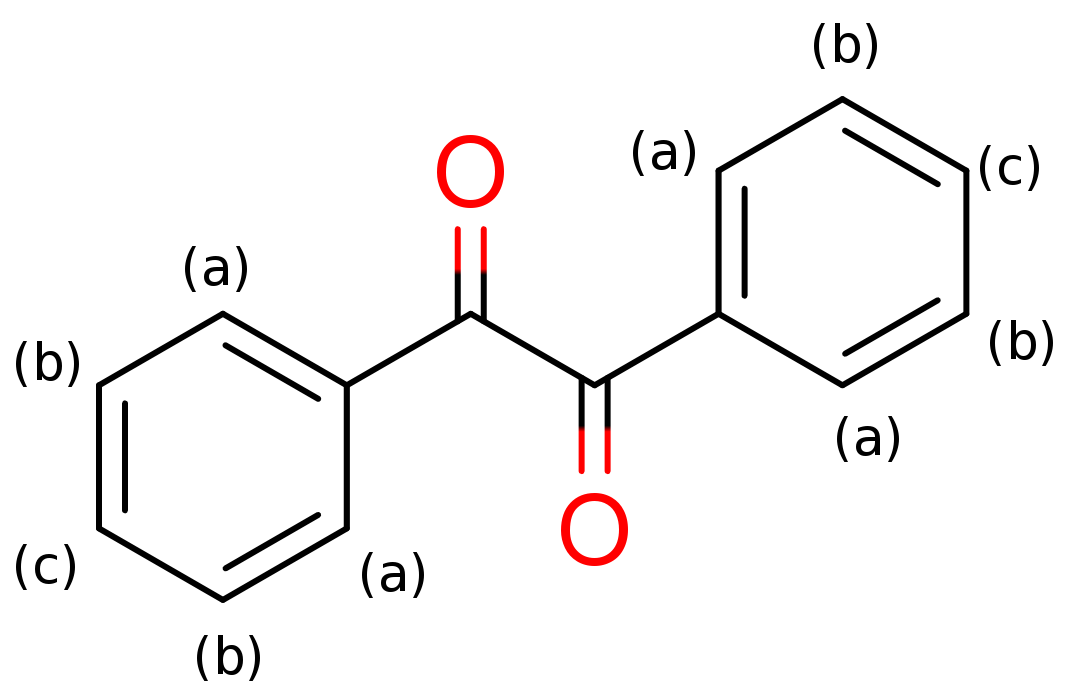
\includegraphics[width=0.5\linewidth]{structures/picosbenzil.png}
\end{scheme}

Adicionalmente el espectro obtenido para el benzil oxidado con acetato de cobre muestra remanentes de benzo\'ina, mientras que el producto de oxidaci\'on con \ce{HNO3} se encuentra puro, como se evidencia en la \autoref{fig: HNMR-Benzil} de la informaci\'on complementaria. A continuaci\'on se discute el mecanismo de oxidaci\'on con cobre, con el objetivo de determinar posibles causas de impureza. 
\begin{scheme}[h]
	\centering
	\caption{Mecanismo de oxidaci\'on de la benzo\'ina por acetato de cobre \cite{wigal2000}.}
	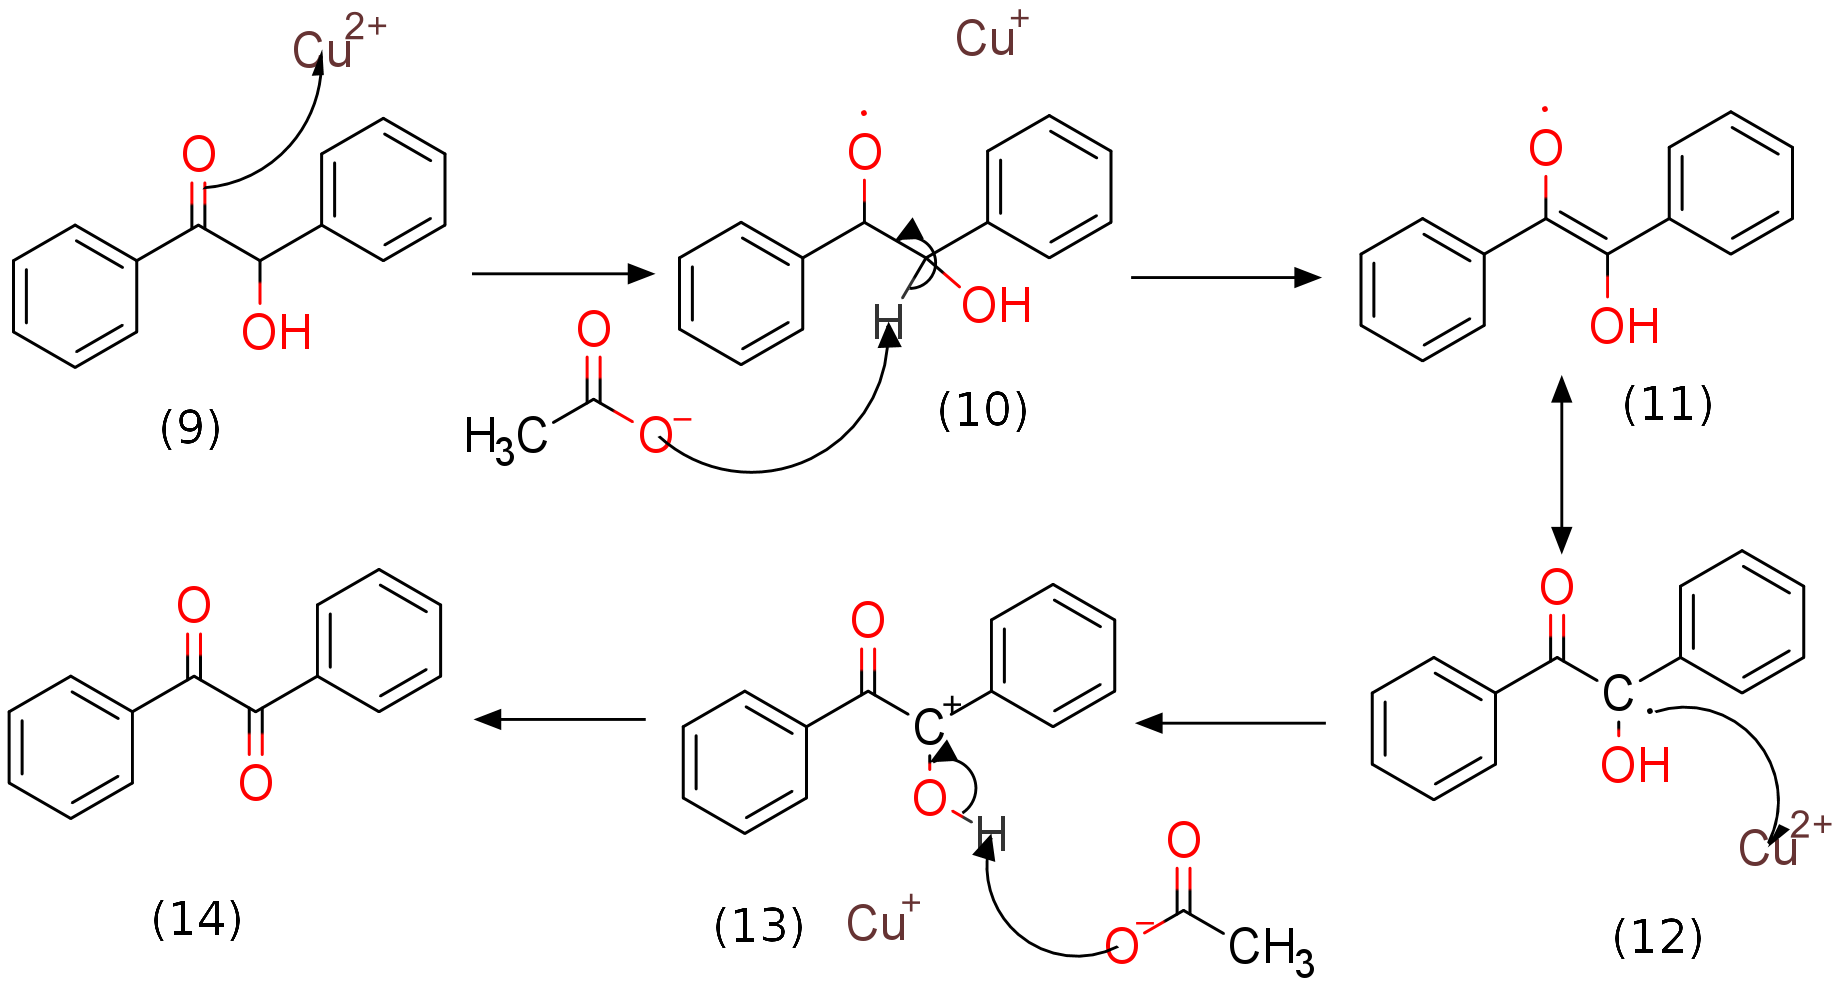
\includegraphics[width=\linewidth]{structures/mechanism-oxidationCu.png}
\end{scheme}

\pagebreak
El acetato de cobre disuelto libera \ce{Cu^2+} el cual es reducido por la benzoina en soluci\'on, dando lugar a un radical sobre la misma \textbf{(9)}. Posteriormente el contraion acetato sustrae el prot\'on del carbono ligado al hidroxilo \textbf{(10)}, dando lugar a un sistema $\pi$ conjugado sobre toda la molecula \textbf{(11)}. Existe un estado resonante con el radical sobre el carbono con la funci\'on alcohol, el cual reduce un \'atomo de cobre (II) circundante \textbf{(12)}. Finalmente una mol\'ecula de acetato ataca el prot\'on del hidroxilo \textbf{(13)}, dando lugar a la formaci\'on del carbonilo \textbf{(14)}.
\begin{scheme}[h]
	\centering
	\caption{Funci\'on catal\'itica del cobre \cite{wigal2000}.}
	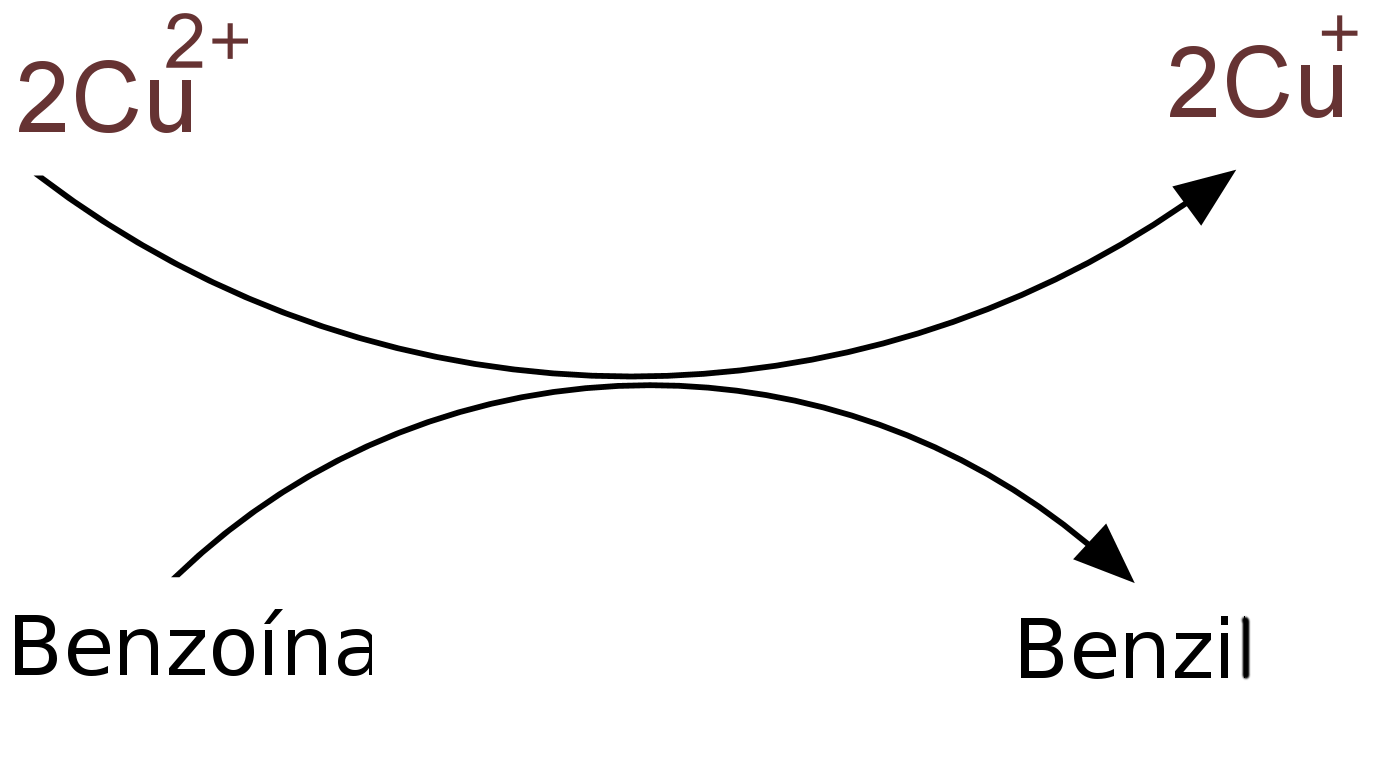
\includegraphics[width=0.5\linewidth]{structures/coppercycle.png}
\end{scheme}

Al realizar la integraci\'on de los hidr\'ogenos en el RMN obtenido, se observa una relaci\'on 2.0:0.5 para los hidr\'ogenos \textit{-para} a la dicetona y el hidr\'ogeno $\alpha$ al carbonilo de la benzo\'ina. Lo anterior implica que existe cerca de 25 \% de benzo\'ina sin reaccionar. Lo anterior se puede explicar si se tiene en cuenta que la oxidaci\'on se lleva a cabo por efecto del cobre, el cual se reduce a cobre (I) y no existe ning\'una sustancia en la reacci\'on que lo oxide de nuevo para continuar con el ciclo catal\'itico. Lo anterior implica que el cobre debe estar en exceso a la benzo\'ina, relaci\'on que no fue tenida en cuenta al momento de realizar el experimento. Una opci\'on es agregar agentes oxidantes a la reacci\'on tales como \ce{NH4NO2}, permitiendo as\'i la continuidad del ciclo catalitico

En el caso del \'acido n\'itrico, es necesaria la formaci\'on del ion \ce{H2NO3+}. El mismo se produce \textit{in situ} bien sea por autoprotonaci\'on del \'acido n\'itrico o la protonaci\'on por el \'acido ac\'etico. El \'acido ac\'etico siendo un \'acido m\'as d\'ebil act\'ua como base y sustrae el prot\'on del \'acido n\'itrico \textbf{(15)}. Posteriormente el ox\'igeno hidroxilo del \ce{HNO3}, ataca al hidr\'ogeno del \'acido ac\'etico protonado \textbf{(16)}. El \'oxigeno del grupo hidroxilo de la benzo\'ina ataca al nitr\'ogeno electrof\'ilico liber\'andose agua, form\'ando el ester con el nitrito \textbf{(17)(18)}. Finalmente el di\'oxido de nitr\'ogeno se elimina con la abstracci\'on del hidr\'ogeno $\alpha$ al carbonilo \textbf{(19)}, dando lugar a la formaci\'on a la dicetona \textbf{(20)}.
\begin{scheme}[h]
	\centering
	\caption{Mecanismo de oxidaci\'on de la benzo\'ina por \'acido n\'itrico \cite{pavia2010}.}
	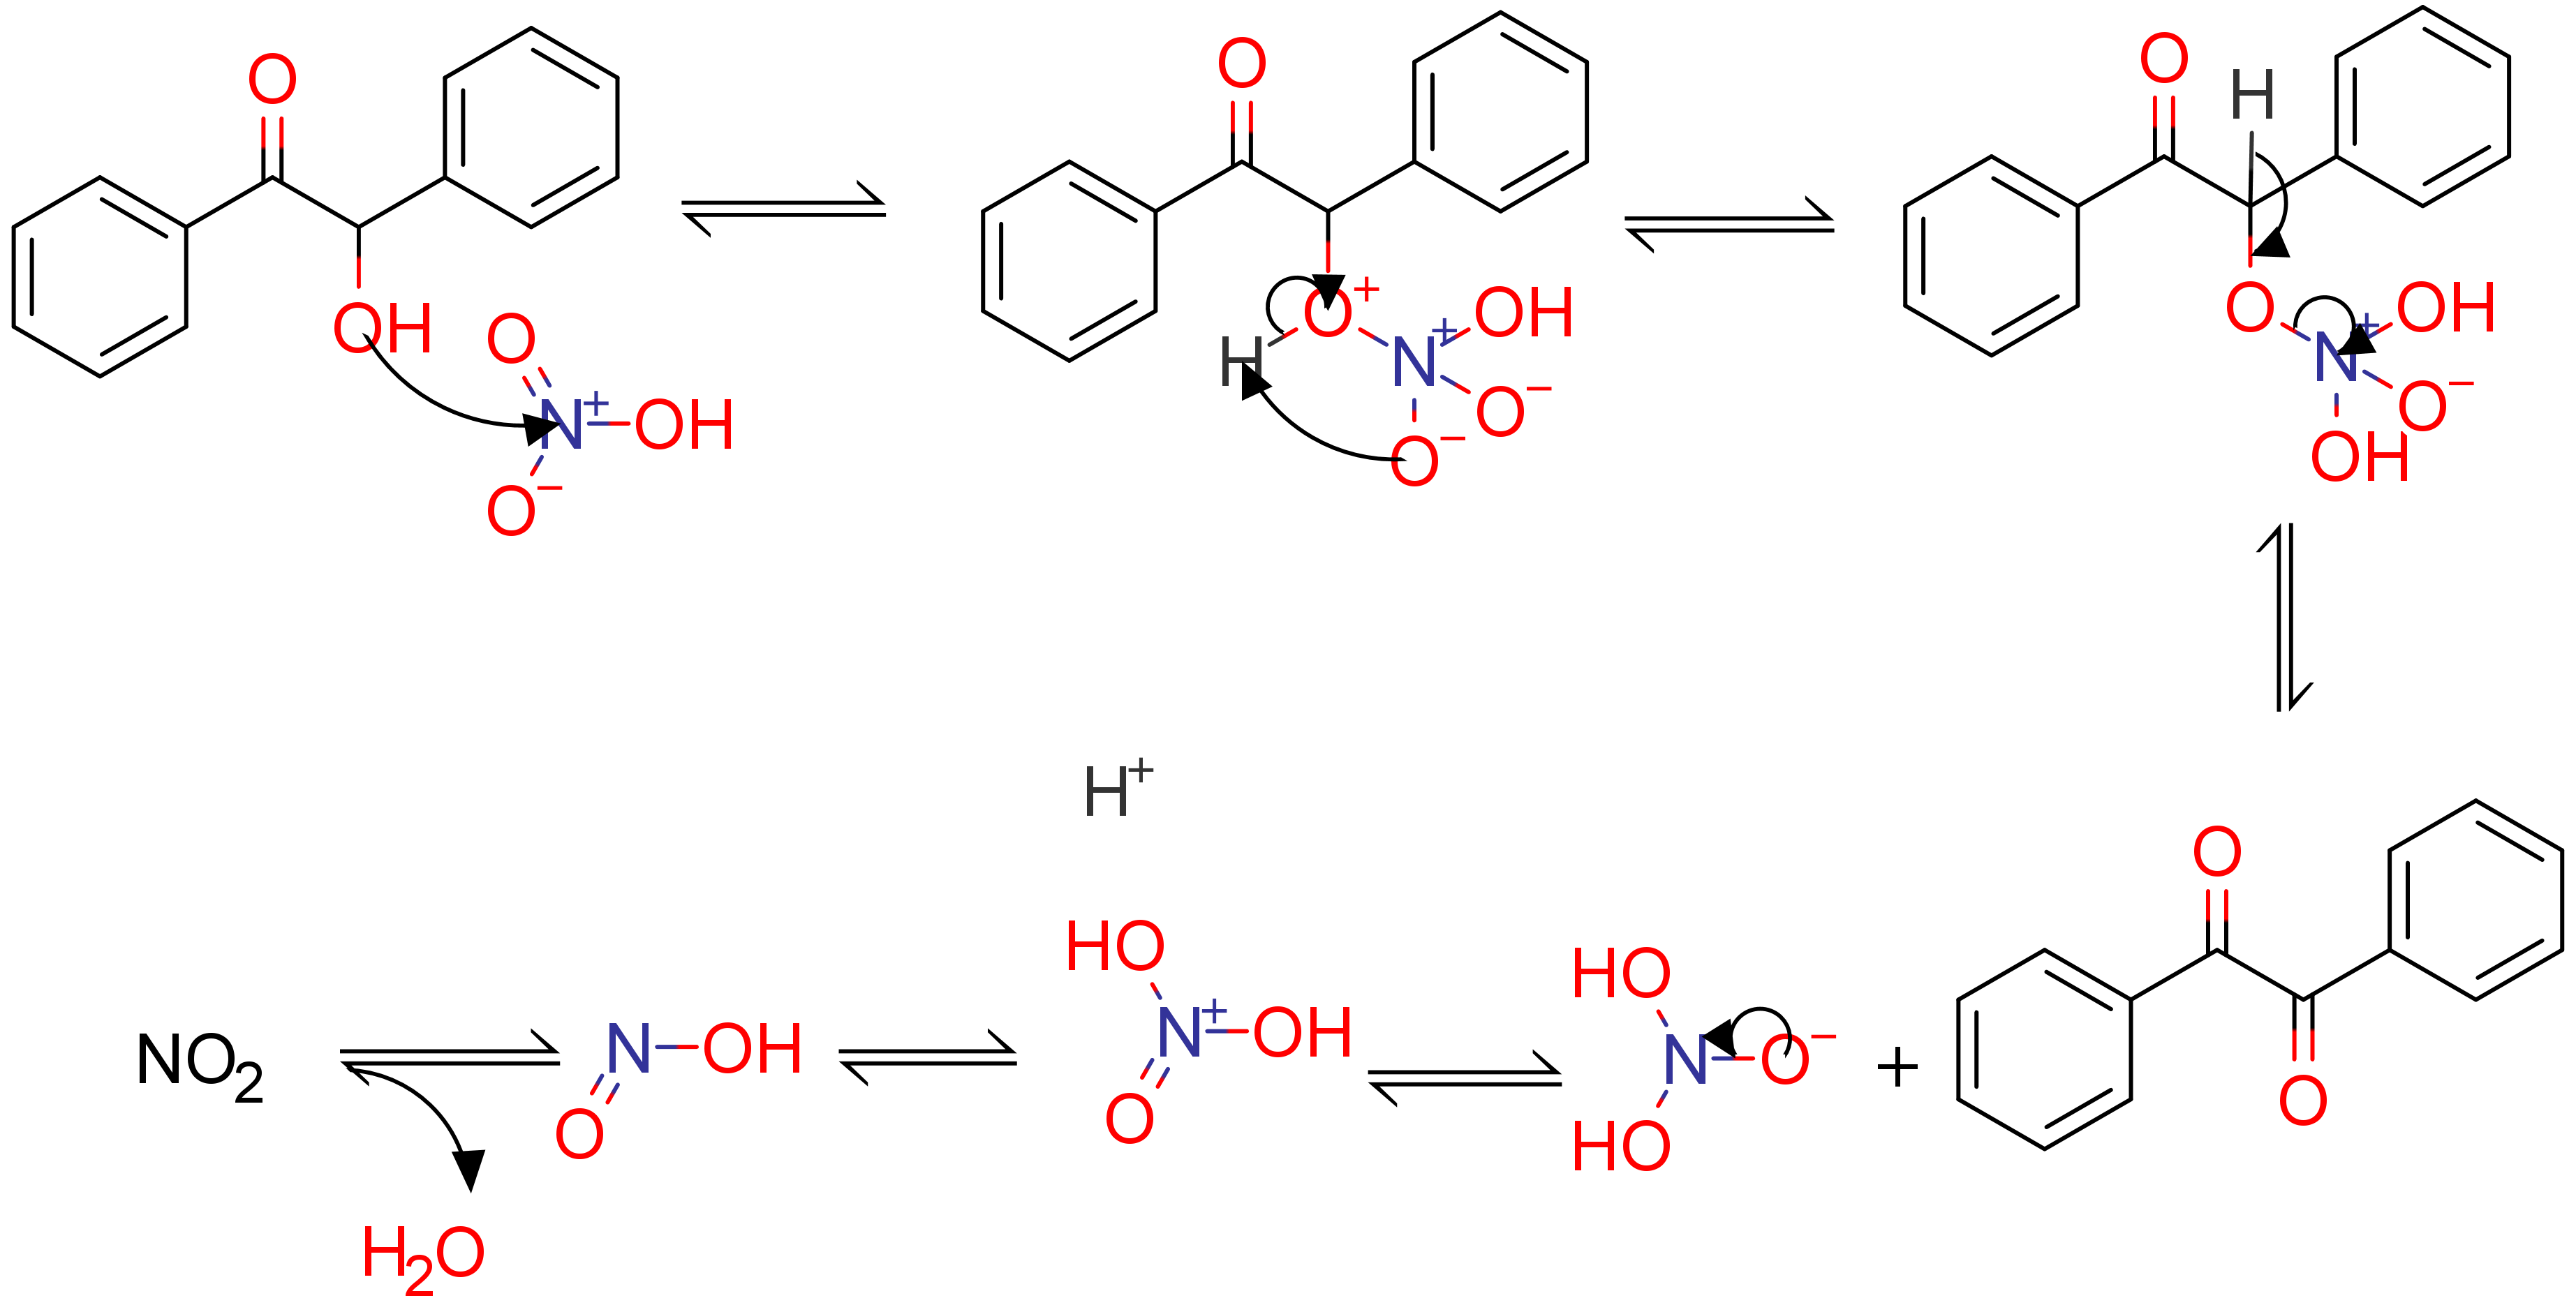
\includegraphics[width=\linewidth]{structures/mechanism-oxidation.png}
\end{scheme}
\pagebreak

La última reacción que se llevó a cabo fue la condensación de urea con benzil en medio básico para obtener la 5,5-difenilhidantoina conocida como Fenitoina y vendida comercialmente bajo el nombre de Dilantin. Existen varios mecanismos propuestos en la literatura, sin embargo, hay dos que predominan y son los que serán mostrados. Ambos comparten una misma etapa inicial y es la deprotonación de la úrea (pKa=15.73 \cite{urea}) por un hidróxido del medio \textbf{(21)} para dar lugar al carbamimidato que luego realiza un ataque nucleofílico sobre el carbonilo del benzil \textbf{(22)} con lo cual se forma un intermediario tetraédrico \textbf{(23)}. Este posteriormente se protona con una molécula de agua del medio \textbf{(24)}, formando el compuesto mostrado en \textbf{(25)}. 
\begin{scheme}[h]
	\centering
	\caption{Primera etapa del mecanismo de condensaci\'on de la \'urea con bezil.}
	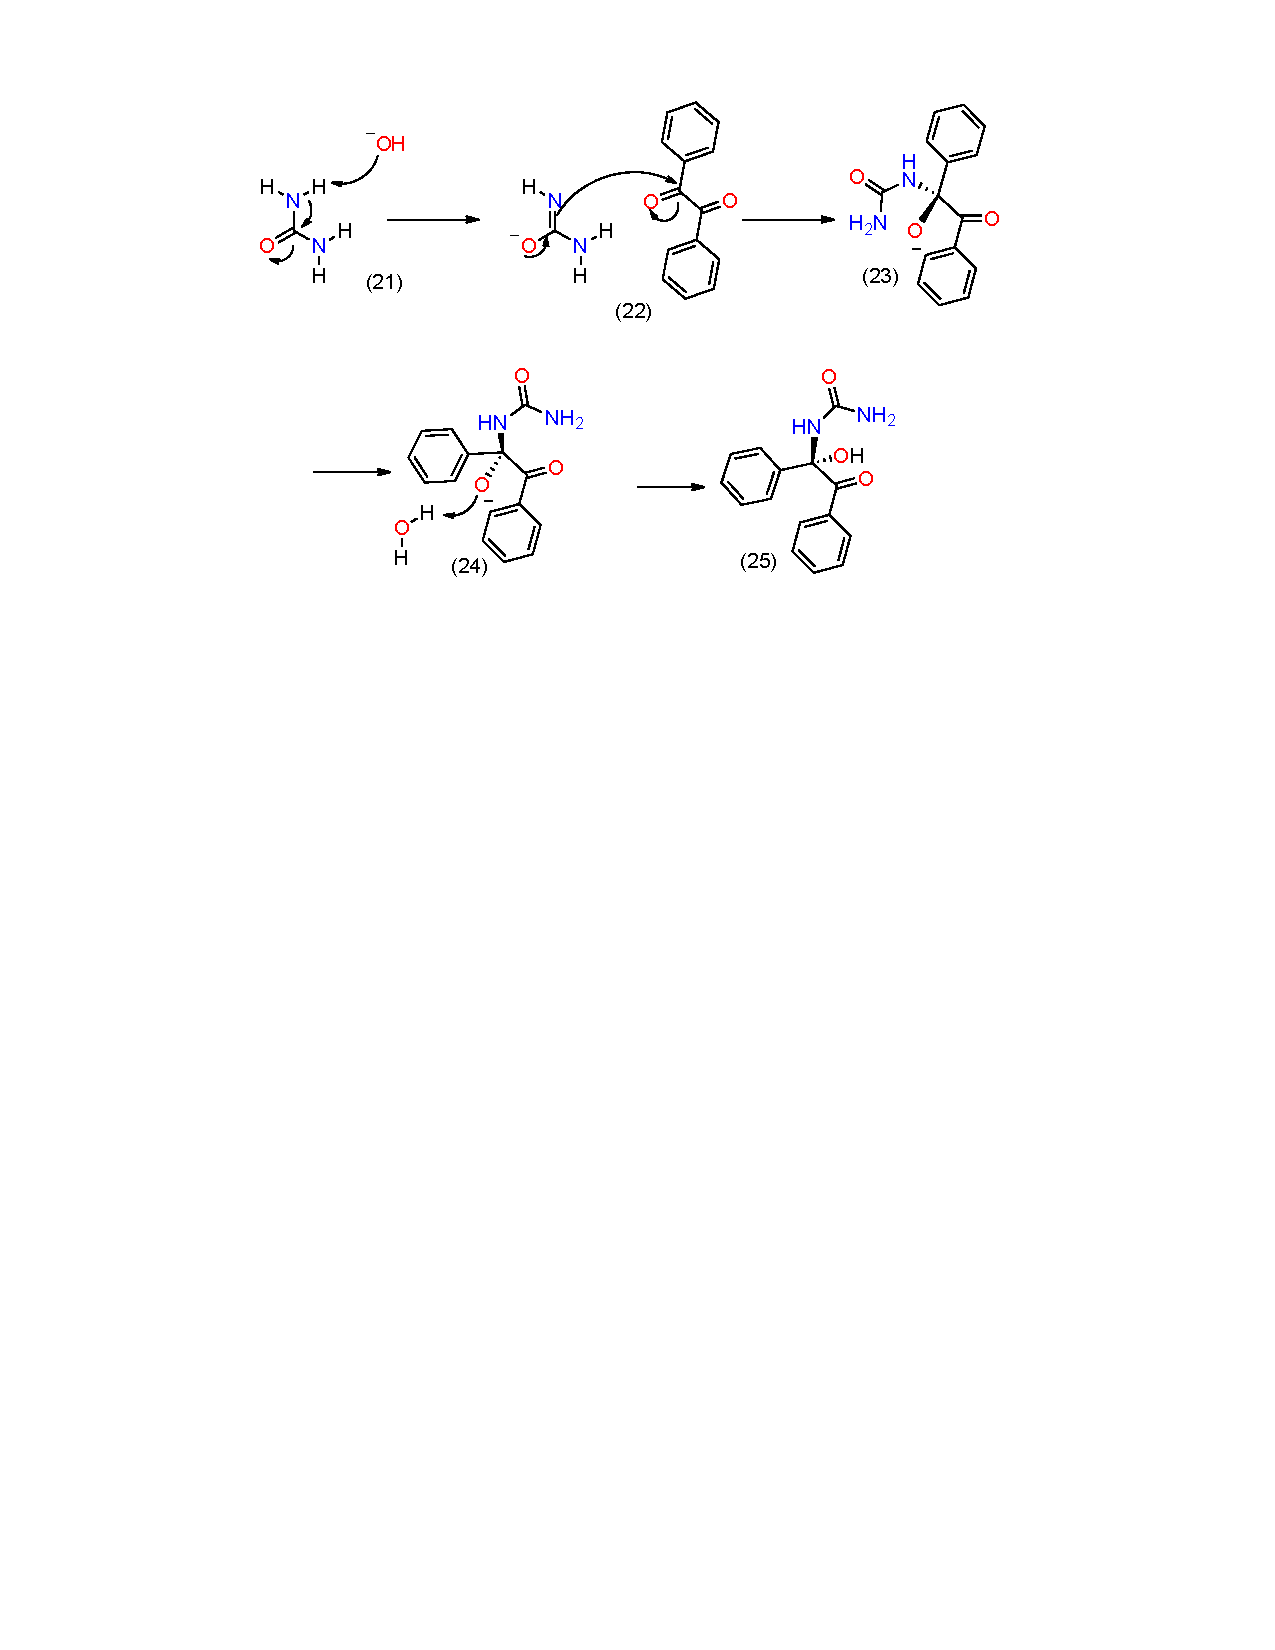
\includegraphics[width=\linewidth]{structures/dilantinesquema1.pdf}
\end{scheme}

Una vez formado el compuesto \textbf{(25)} se puede llevar a cabo dos deprotonaciones distintas que dan lugar a los dos diversos mecanismos. En el primer caso un hidróxido reacciona con el hidrógeno de la amida secundaria \cite{dunnavant1956}\cite{hayward1983} \textbf{(26)}, para formar un carbamimidato \textbf{(27)}. El par electrónico sobre el oxígeno regenera el carbonilo dando lugar a la formación de una imina \textbf{(28)}. Una vez más el hidróxido deprotona la urea y el carbamimidato formado realiza un ataque nucleofílico sobre el carbonilo restante \textbf{(29)} dando lugar a la formación de un ciclo de cinco miembros \textbf{(30)}. Posteriormente el par electrónico de alcóxido forma un carbonilo, lo cual sirve de fuerza motriz para el rearreglo bencílico que da lugar a la formación de dos fenilos geminales \textbf{(31)}. Luego el nitrógeno de la amida se protona para dar lugar al producto final \textbf{(32)}, sin embargo como se está en medio básico se deprotona la imida (pKa imida = 14.7, pKa amida = 26.9 en DMSO \cite{bordwellpkatableacidityindmso}) formando la especie \textbf{(33)}. Una vez realizado el workup ácido se vuelve a protonar la molécula y se obtiene finalmente la 5,5-difenilhidantoina \textbf{(34)}.
\begin{scheme}[h]
	\centering
	\caption{Caso uno, de la condensaci\'on entre la \'urea y el benzil.}
	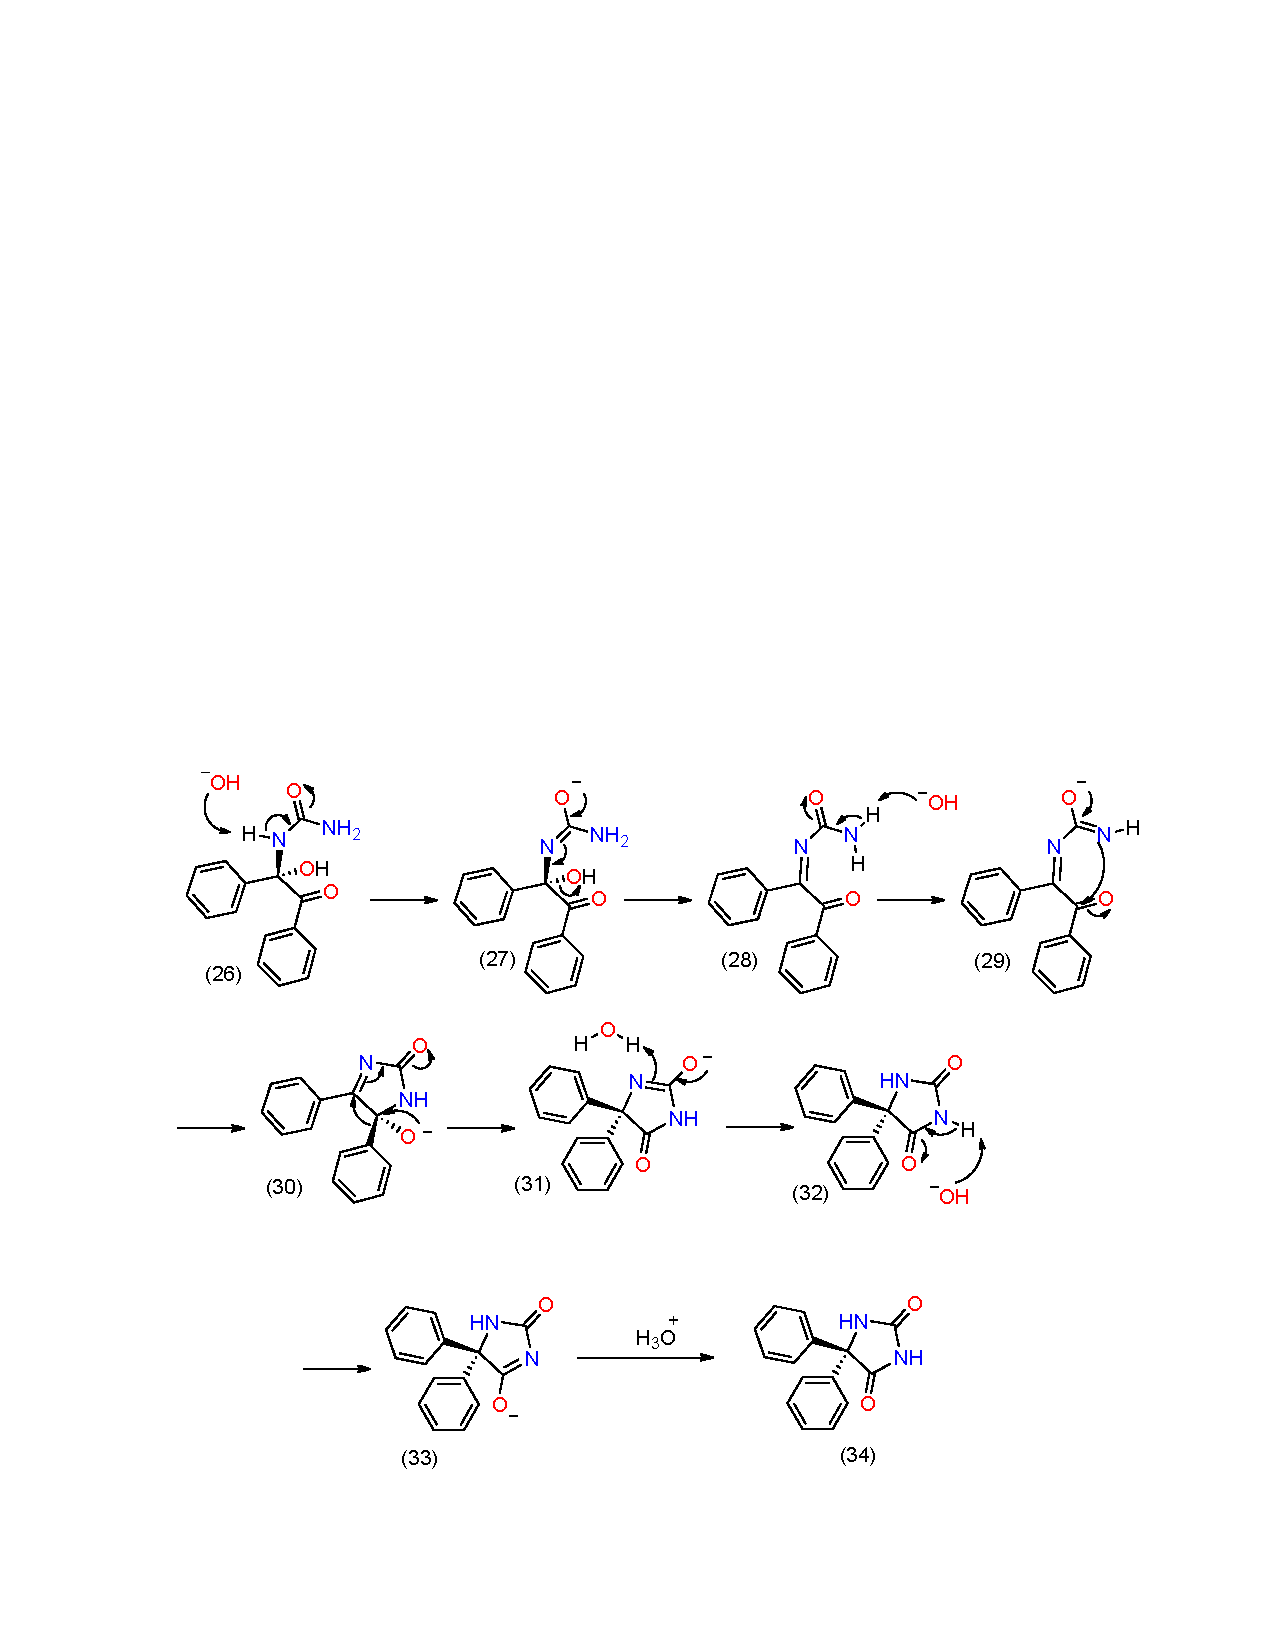
\includegraphics[width=\linewidth]{structures/dilantinesquema2.pdf}
\end{scheme}

%\pagebreak
En el caso del segundo mecanismo propuesto el hidróxido en vez de deprotonar la amida secundaria \cite{mahmoodi2004}\cite{gbaguidi2011}, reacciona con la amida primaria \textbf{(35)} formando el carbamimidato que realiza un ataque nucleofílico sobre el carbonilo \textbf{(36)} formando una imidazolidina \textbf{(37)}. Esta es deprotonada por un hidroxilo del medio, de modo que se genera una carga negativa sobre el oxígeno \textbf{(38)} el cual al formar el carbonilo da lugar a la eliminación de un hidroxilo y la formación de una imina \textbf{(39)}. El alcóxido en \textbf{(39)} da lugar a la formación de un carbonilo y genera la migración del fenilo a la imina (rearreglo bencílico). De manera similar que en las etapas \textbf{(31-34)} del primer mecanismo propuesto se da la protonación y deprotonación de la amida e imida respectivamente, hasta que finalmente con el workup ácido se obtiene el producto final.
\begin{scheme}[h]
	\centering
	\caption{Caso dos, de la condensaci\'on entre la \'urea y el benzil.}
	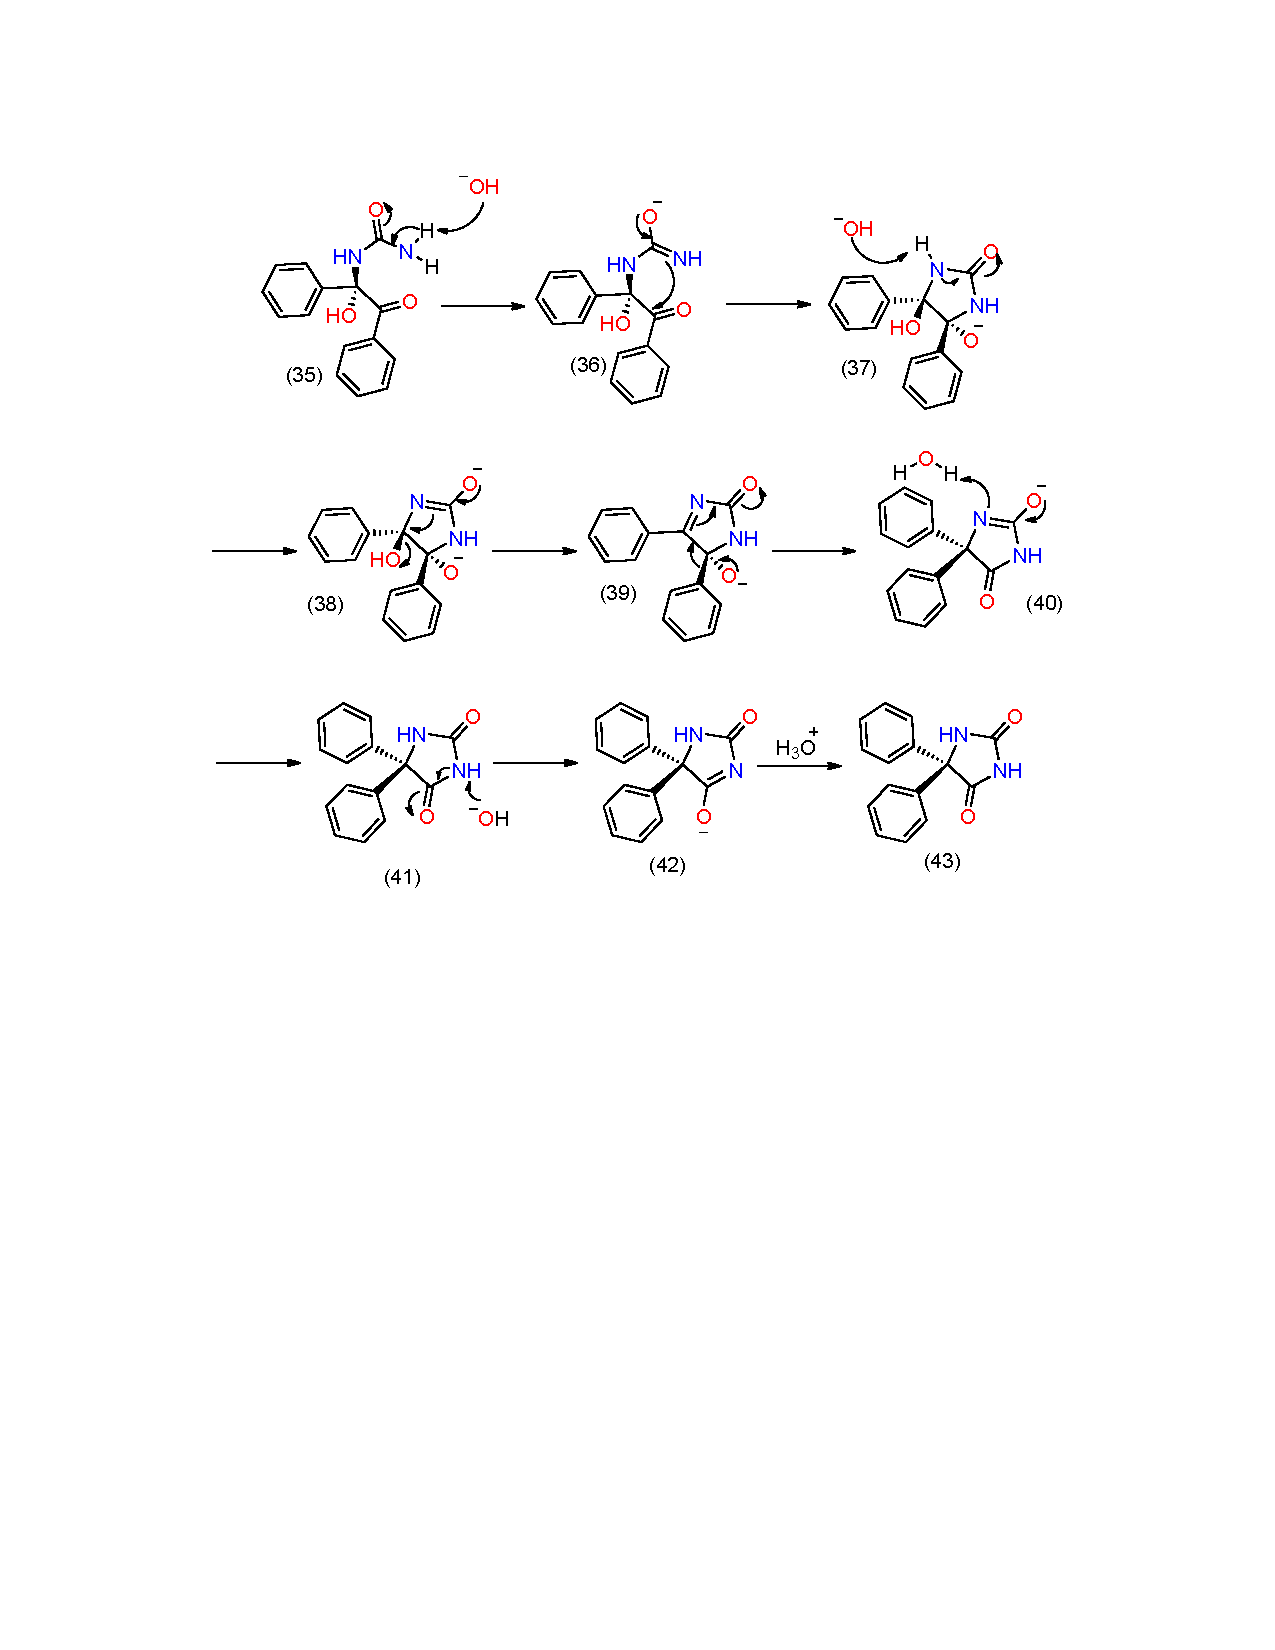
\includegraphics[width=0.95\linewidth]{structures/dilantinesquema3.pdf}
\end{scheme}

El rearreglo bencílico que se da entre \textbf{(30)-(31)} y \textbf{(38)-(39)} es de particular interés ya que involucra la migración de un carbanión , el cual es un proceso poco común en comparación a los rearreglos de carbocatión \cite{comisar2007}. Durante mucho tiempo hubo incertidumbre sobre el mecanismo de la transposición [1,2] de un carbanión, esto se debe a que según la teoría de orbitales moleculares está prohibida por simetría ya que el carbanión se encuentra fuera de fase con respecto a los orbitales p de los carbonos involucrados \cite{yamabe2006}\cite{burke2007} (\autoref{fig: figuran}).
\begin{figure}[h]
	\centering
	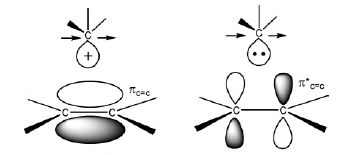
\includegraphics[width=\linewidth]{figuran.png}
	\caption{Orbitales p de los carbonos involucrados \cite{yamabe2006}.}
	\label{fig: figuran}
\end{figure}

Sin embargo en el caso de las 1,2-dicetonas (al igual que en la imina y carboxilo que se forma en \textbf{(30)-(31)} y \textbf{(38)-(39)})  el sistema de orbitales involucrados no es únicamente el de los carbonos dentro de los cuales se da la migración, sino que toca tener en cuenta los orbitales del carbonilo \autoref{fig: figuran1} (o imina). De este modo al combinar los orbitales moleculares se obtiene un LUMO enlazante, este lóbulo sin nodos permite la fácil migración de carbanión \cite{yamabe2006}. En consecuencia los carbonos C1 - C2 de la 1,2-dicetona (o también del sistema con la imina) no funcionan como un centro electrofílico sino que como parte de un sistema de 4 electrones $\pi$, de modo que con el carbanión se tiene un sistema 4+2 electrones \cite{yamabe2006}\cite{burke2007}. Este cumple con las reglas de Woodward-Hoffman y el proceso es permitido por la conservación de la simetría del orbital \cite{yamabe2006}.
\begin{figure}[h]
	\centering
	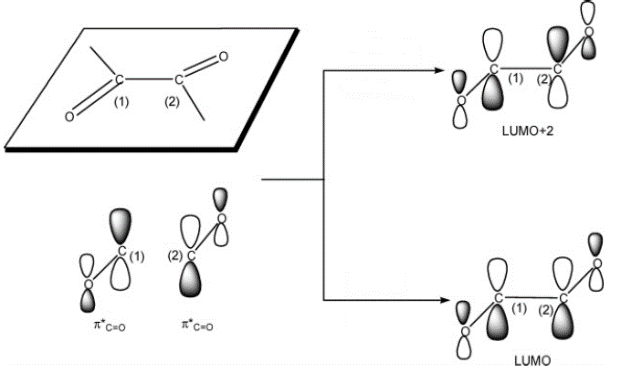
\includegraphics[width=\linewidth]{figuran1.png}
	\caption{Conservaci\'on de la simetr\'ia de orbitales en la reacci\'on \cite{yamabe2006}.}
	\label{fig: figuran1}
\end{figure}

Estudios computacionales del rearreglo del benzil a ácido bencílico indican que todas las etapas de la reacción son exotérmicas a excepción del ataque nucleofílico, la isomerizaci\'on y la migración del fenil. Esta última tiene un cambio de energía considerablemente más grande ($\Delta E=10.41$ kcal/mol) que la adición nucleofílico ($\Delta E = 0.29$ kcal/mol) y por lo tanto es el paso determinante de la reacción \cite{yamabe2006}. Considerando que la condensación de benzil con urea sigue un proceso similar, se asume que este también será el paso determinante para la síntesis de Dilantin a partir de benzil. También se evidenció que el solvente influye sobre la velocidad de reacción de dos modos, el primero es que está involucrado en la adición del nucleófilo a uno de los carbonilos, facilitando la aproximación de este al LUMO del sistema \autoref{fig: figuran2}. El segundo consiste en que el solvente (DMSO) favorece la delocalización de carga en el fenil durante el rearreglo, facilitando dicho proceso.
\begin{figure}[h]
	\centering
	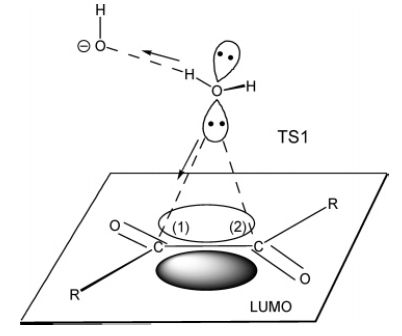
\includegraphics[width=0.6\linewidth]{figuran2.png}
	\caption{Adici\'on del nucle\'ofilo \cite{yamabe2006}.}
	\label{fig: figuran2}
\end{figure}

Enfocándonos un poco más en el estado de transición de la migración del fenil (\autoref{fig: figuran3}) esta se caracteriza por ser un puente triangular \cite{yamabe2006}\cite{bowden1994} donde el anión se aproxima de forma perpendicular al plano donde se encuentran los carbonos C1 - C2.  Solo con esta geometría es posible que los orbitales p de los carbonos C1 - C2 interactúen con el orbital ocupado sp$^2$ del fenil confiriendo mayor estabilidad. En el estado de transición, el fenil que no migra es coplanar a los carbonos C1 - C2 y la conjugación se expande a todo el plano del ácido $\alpha$-oxo-carboxílico \cite{yamabe2006}. Dicha simetría del estado de transición es similar para el caso del rearreglo en \textbf{(30)-(31)} y \textbf{(38)-(39)}, la única diferencia es que en vez de involucrar los orbitales p del carbonilo se utilizan los orbitales p del carbono de la imina.
\begin{figure}[h]
	\centering
	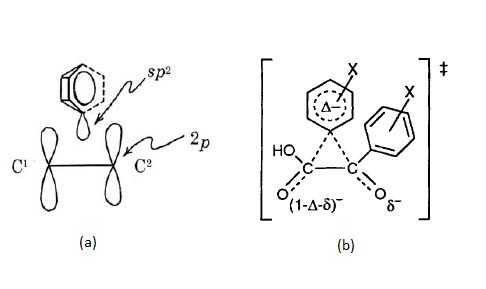
\includegraphics[width=\linewidth]{figuran3.png}
	\caption{Migraci\'on del fenil \cite{phelan1967}.}
	\label{fig: figuran3}
\end{figure}

Para esta síntesis se utilizaron dos metodologías diferentes, una siguiendo la síntesis clásica por medio de la condensación de urea y benzil en reflujo \cite{dunnavant1956}\cite{triovi2015}\cite{safari2010}, y la otra realizando condensación de urea y benzil por medio de ultrasonido \cite{safari2010}.  Las ventajas de esta última, según lo reportado en el artículo, eran altos rendimientos (98\%), alta pureza del producto y cortos tiempos de reacción (3 min) \cite{safari2010}. De este modo se esperaba obtener mejores resultados con el ultrasonido que con el reflujo, sin embargo al analizar los espectros $^1$H-RNM se evidenció lo contrario. En ambos casos se identificaron las mismas señales, pero con proporciones distintas.  El singlete en 11.16 ppm corresponde al hidrógeno de la imida (b) (\autoref{sc: dilantin}), altamente desprotegido por el efecto inductivo de los carbonilos. El hidrógeno de la amida (a) es un singlete en 9.37 ppm y los hidrógenos aromáticos se ven entre 7.5 – 7.25 ppm.
\begin{scheme}[h]
	\centering
	\caption{Asignaci\'on de protones para el Dilantin.}
	\label{sc: dilantin}
	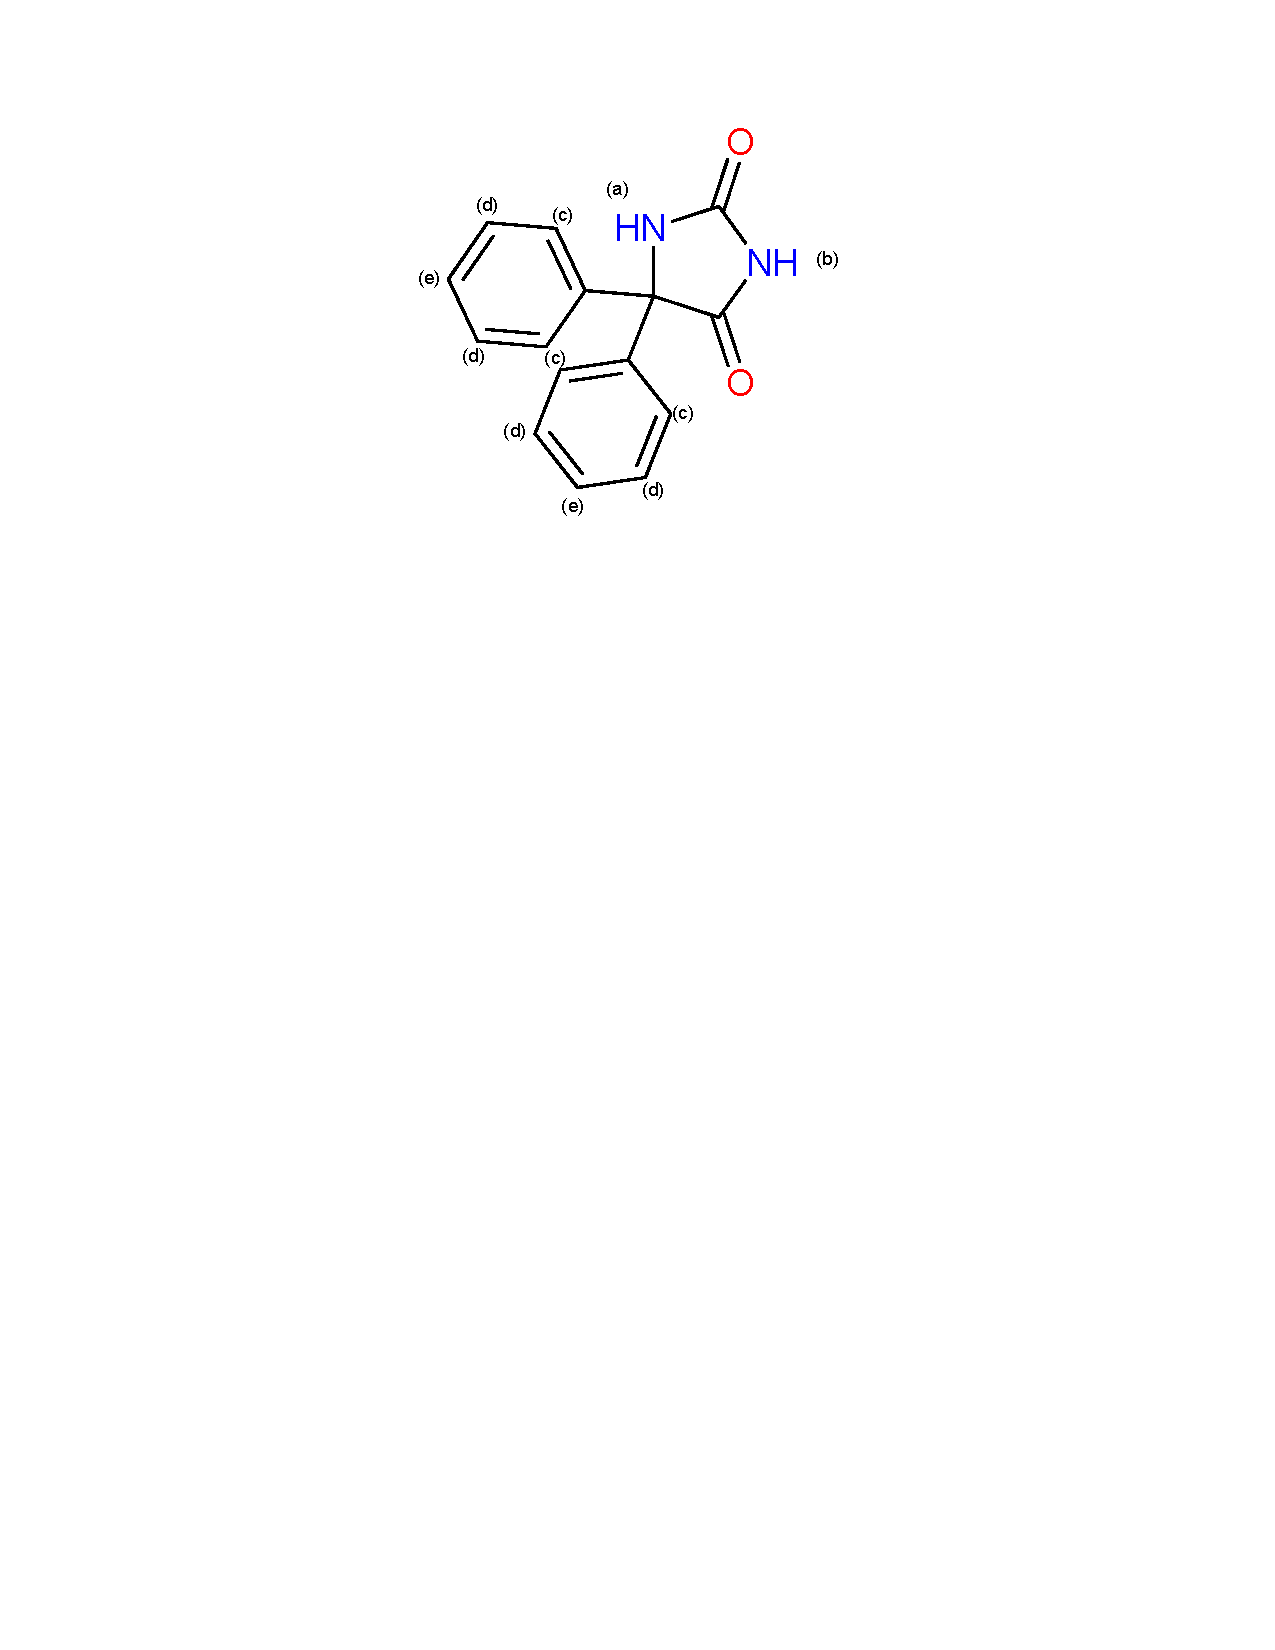
\includegraphics[width=0.5\linewidth]{structures/picos1.pdf}
\end{scheme}

Sin embargo, se encuentran otras señales en 7.81 ppm y entre 7.10-7 ppm. Dichas señales corresponden a la impureza que se obtiene por medio doble condenzación de urea con benzil, formando 7,8-difenilglicoluril (\autoref{sc: otro}). El singlete en 7.81 ppm corresponde a los hidrógenos de la amida (a), mientras que el multiplete entre 7.10 y 7 ppm corresponde a los hidrógenos aromáticos. La señal en 2.51 ppm corresponde al solvente (DMSO).
\begin{scheme}[h]
	\centering
	\caption{Asignaci\'on de protones para el 7,8-difenilglicoluril.}
	\label{sc: otro}
	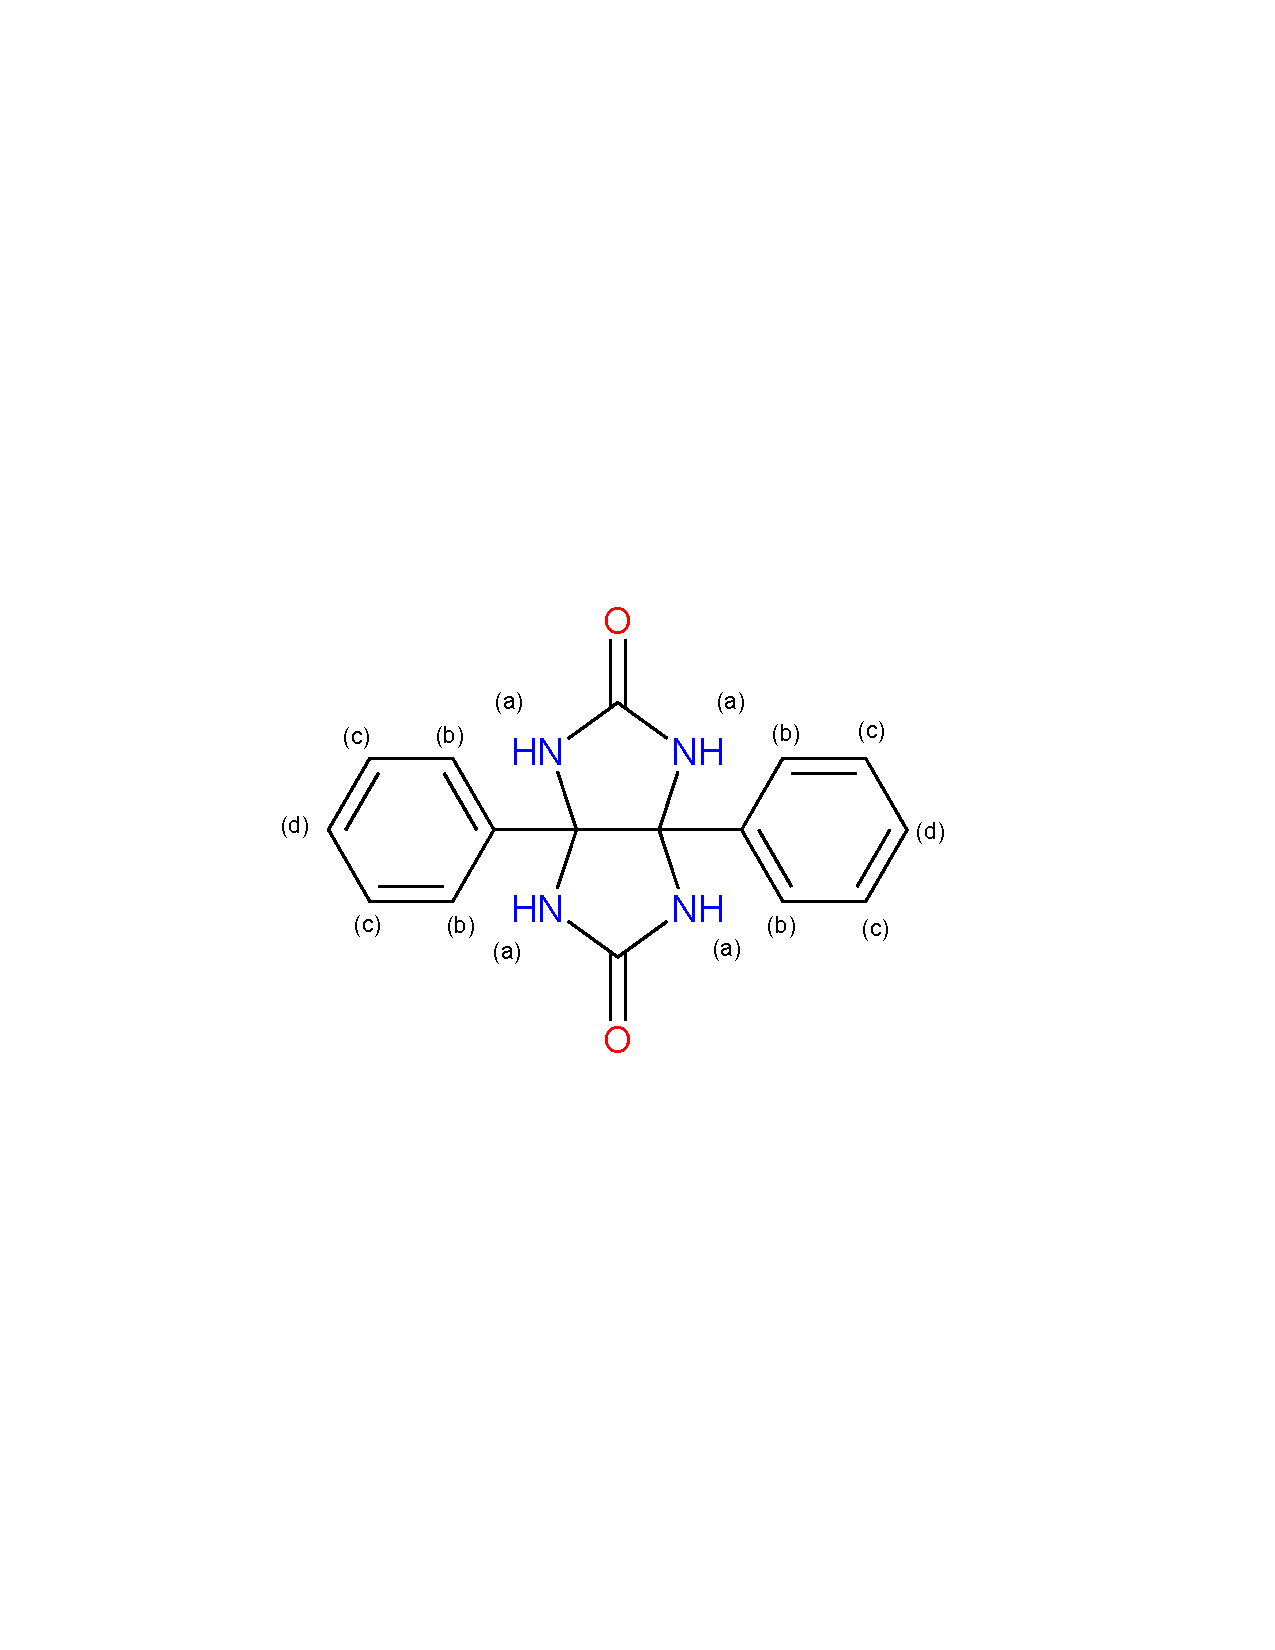
\includegraphics[width=0.7\linewidth]{structures/picos2.pdf}
\end{scheme}

Al comparar la integración de las señales para el Dilantin y el 7,8-difenilglicoluril tanto en el caso de la condensación en reflujo como ultrasonido se encontró que en el primer caso la proporción Dilantin:glicoluril es de 1:0.13, mientras en el segundo es de 1:0.57. De este modo la síntesis por ultrasonido dio una menor pureza del producto en comparación al método clásico. La causa puede ser que las burbujas que colapsan en ultrasonido generan puntos calientes localizados (con altas presiones y temperaturas) con cortos periodos de vida, lo que induce la fragmentación molecular y formación de especies altamente reactivas \cite{li2010}, lo que también podría justificar las pequeñas impurezas que se ven en el RMN.

En la literatura no se muestra el mecanismo de la formación del 7,8-difenil glicoluril como subproducto, se propone que esta se da por la doble condensación de la urea aun estando en medio básico, pero no se hace más énfasis en esto. El compuesto de partida es el dialcóxido obtenido después de la primera condensación de la úrea \cite{li2010}\cite{sachdev2010} el cual está en equilibrio con su versión protonada, el diol. Todo comienza cuando el hidróxido del medio remueve el hidrógeno de una amida \textbf{(34)} lo cual da lugar a la formación del compuesto \textbf{(35)}. Al delocalizarse los electrones del oxígeno para dar lugar al carboxilo, se forma una imina, la cual sufre un ataque nucleofílico por parte del carbamimidato \textbf{(36)}. Posteriormente la amida se vuelve a protonar \textbf{(37)} y se repite el proceso de deprotonación \textbf{(38)}, eliminación de hidroxilo \textbf{(39)}, formación \textbf{(40)} y ataque del carbamimidato \textbf{(41)} y protonación de la amida \textbf{(42)}, para dar lugar al producto de la doble condensación de la urea.
\begin{scheme}[h]
	\centering
	\caption{Mecanismo final para el subproducto del rearreglo.}
	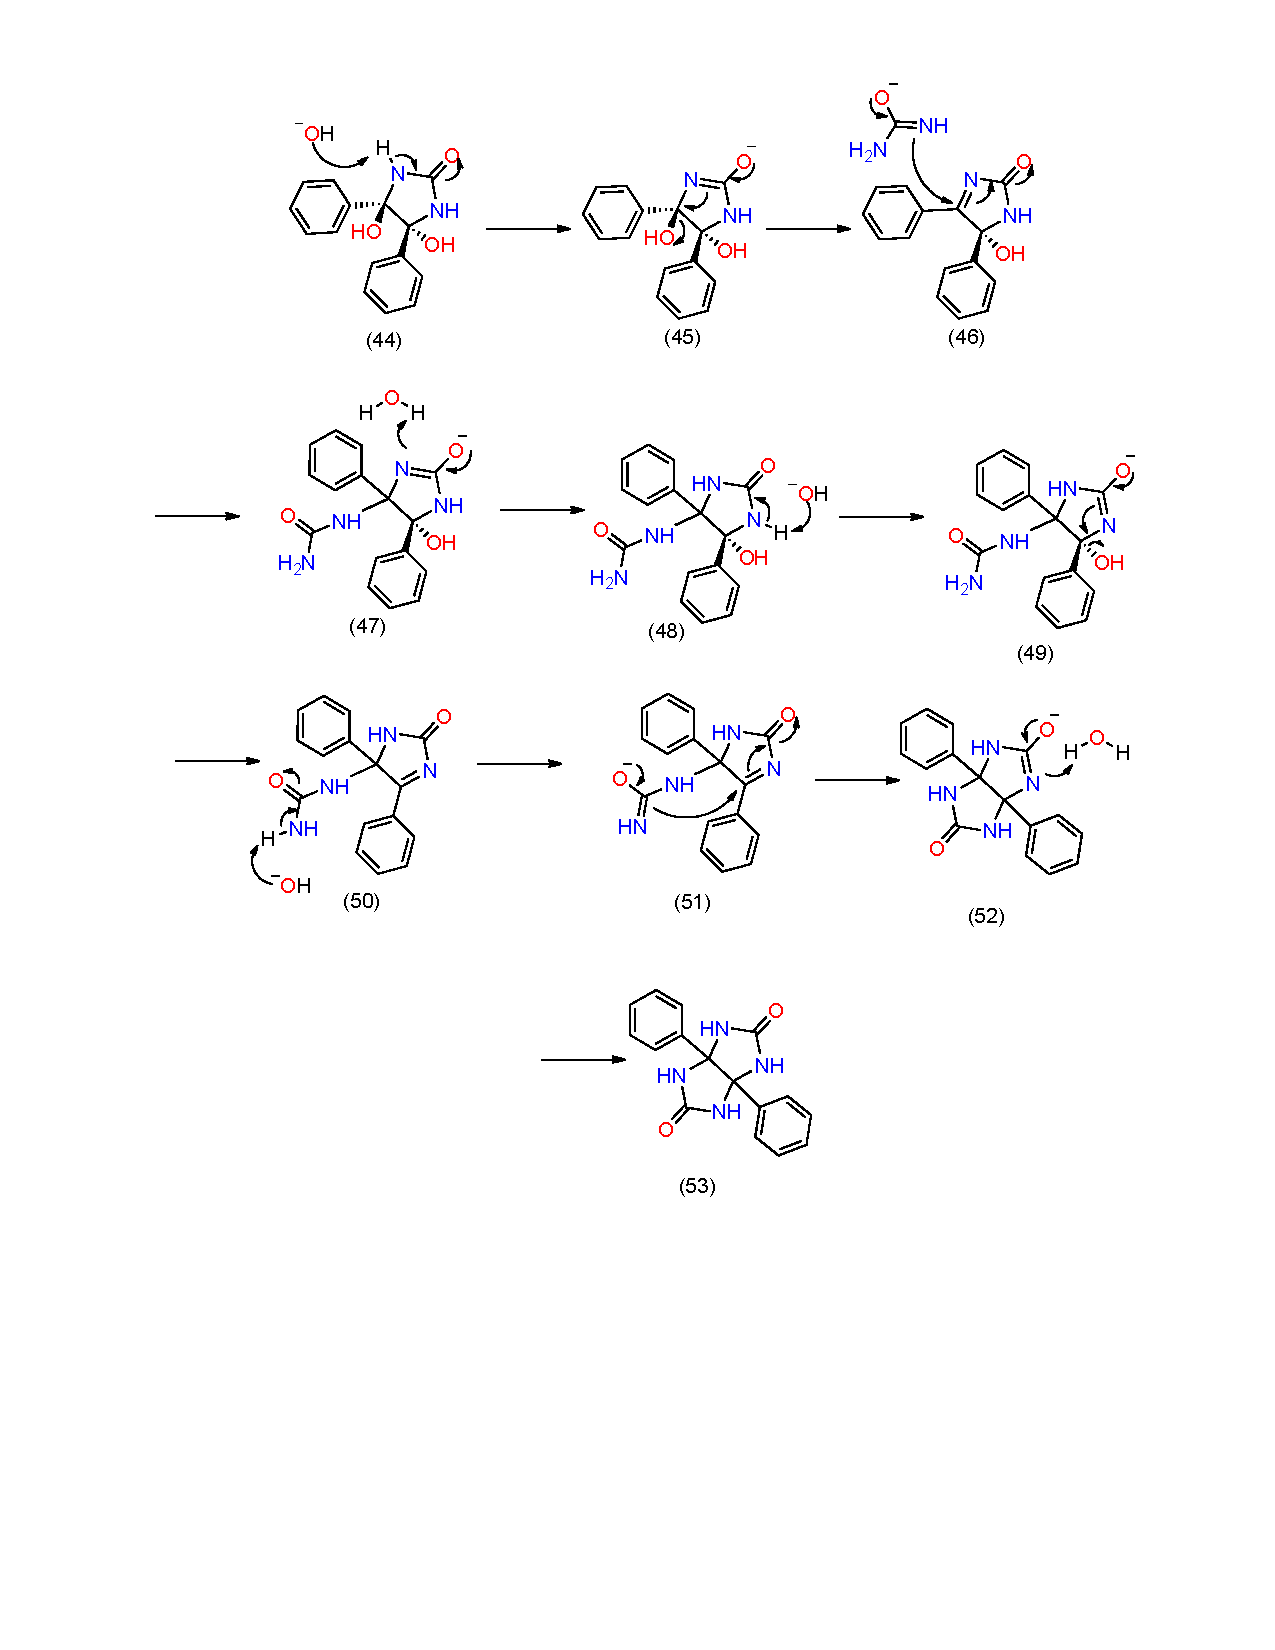
\includegraphics[width=\linewidth]{structures/subproducto_esquema_4.pdf}
\end{scheme}

Un problema con este mecanismo es que la imina es menos electrofílica que el carboxilo debido a la diferencia de electronegatividad del oxígeno y el nitrógeno, por lo que puede que el ataque nucleofílico del carbamimidato de la urea no sea tan favorable. Sin embargo, la imina está directamente unida a un carboxilo por parte del nitrógeno y su estructura asemeja bastante a la de un aceptor de Michael. De hecho, el nitrógeno al ser más electronegativo que el carbono generaría una deficiencia de carga mayor sobre el carbono $\beta$ aumentando de este modo el coeficiente del orbital LUMO. En consecuencia, favoreciendo el ataque nucleofílico a esta posición.
\begin{scheme}[h]
	\centering
	\caption{Resonancia en la imina.}
	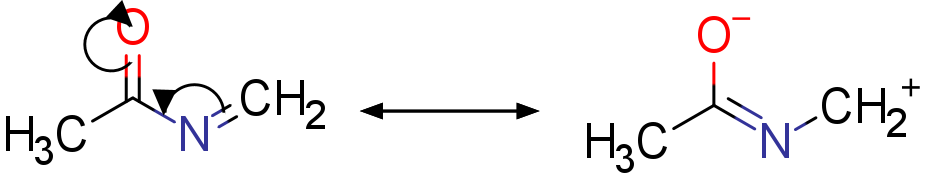
\includegraphics[width=0.6\linewidth]{structures/resonancia.png}
\end{scheme}

Una ventaja del mecanismo propuesto es que explicaría por qué al aumentar la alcalinidad del medio la cantidad de glicoluril disminuye \cite{dunnavant1956}. Esto se debe a que entre más básico esté el medio, menor será la proporción de diol \textbf{(34)} y mayor la de alcóxido. Con el alcóxido no se pude llevar a cabo la reacción ya que el \ce{O^2-} no es un grupo saliente viable. Otra opción es que al hacer el workup con ácido se forme el diol \textbf{(34)} y este se condense con la urea en medio ácido, como lo indica el mecanismo en el \autoref{sc: ultimo}. Sin embargo este mecanismo no explicaría como afecta la concentración de base en la proporción de hidantoina-glicoluril y se esperaría ver, así sea en pequeñas proporciones, otros subproductos como por ejemplo éteres producto del ataque por parte del etanol (la proporción de este que no esté protonado).
\begin{scheme}[h]
	\centering
	\caption{Mecanismo final para el subproducto del rearreglo.}
	\label{sc: ultimo}
	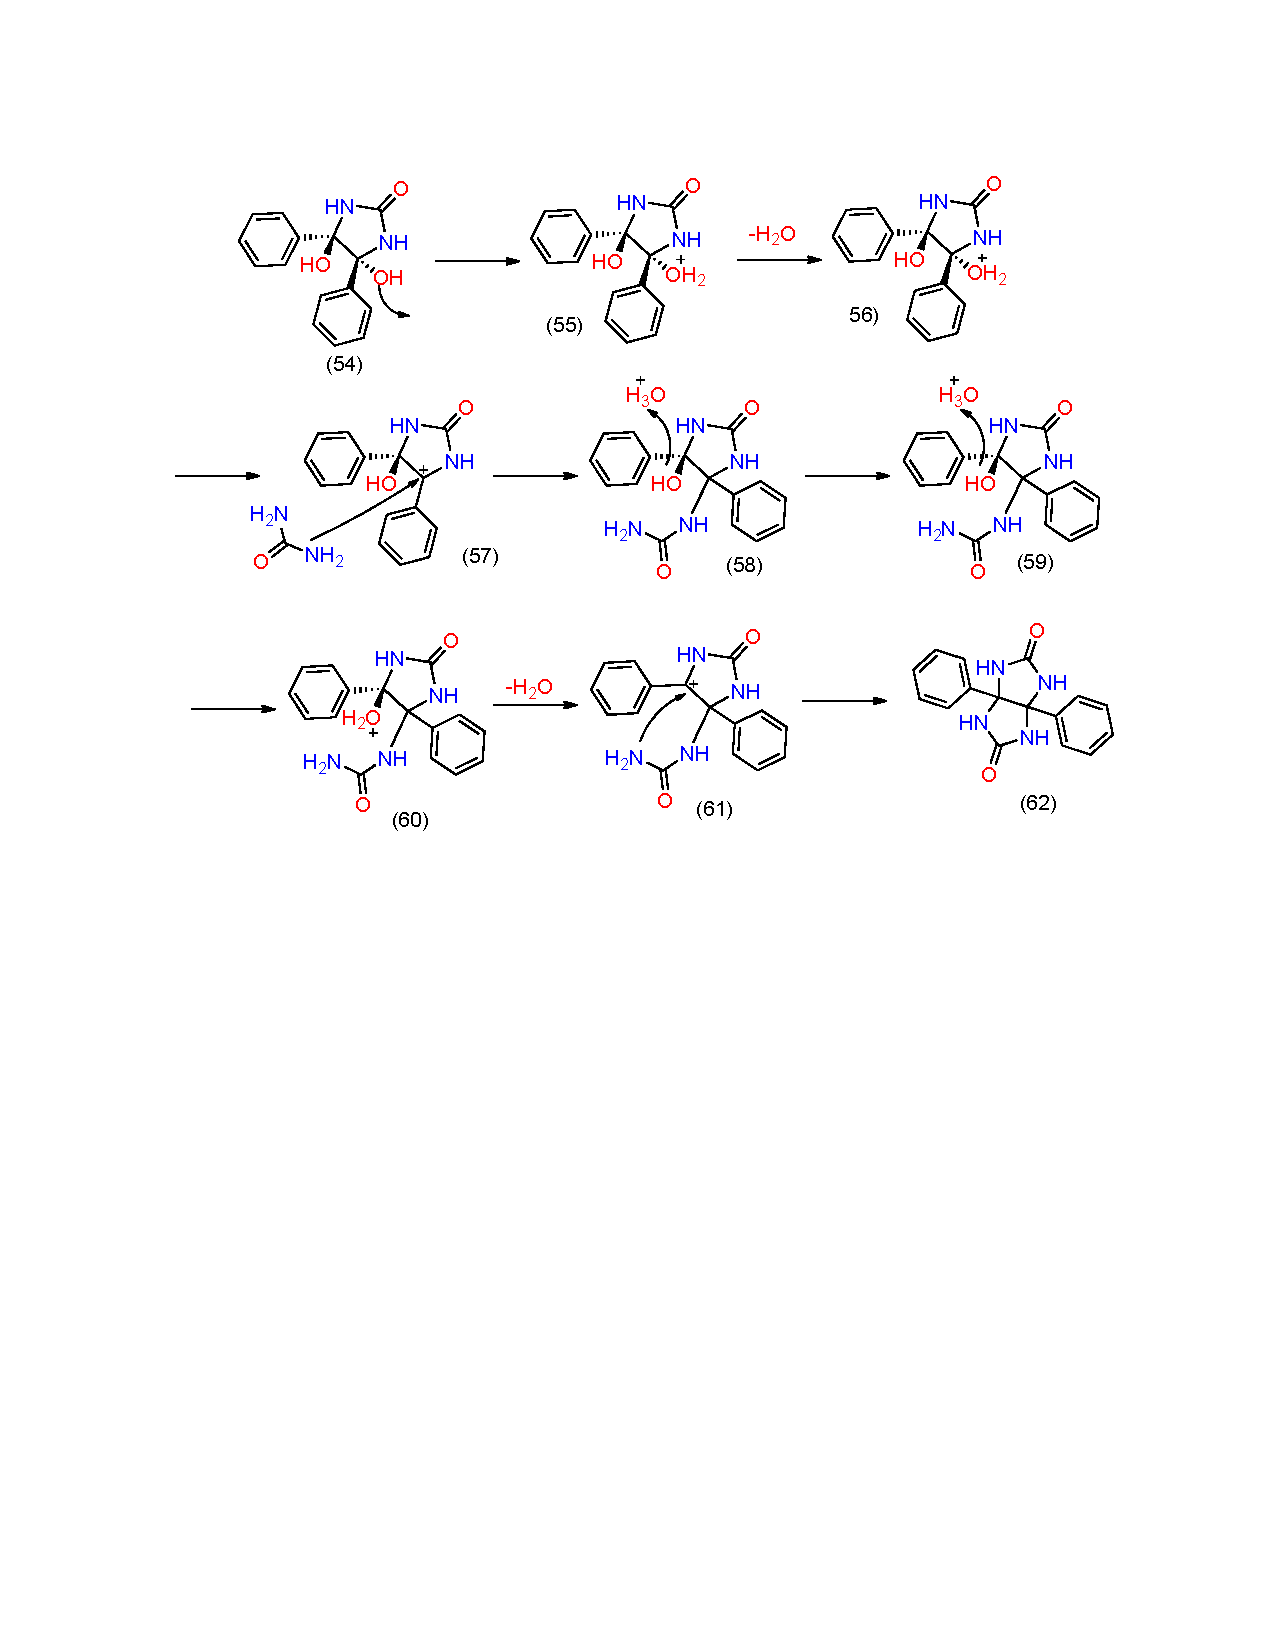
\includegraphics[width=\linewidth]{structures/subproducto_ultimo_esquema.pdf}
\end{scheme}

\section{Conclusiones}
La s\'intesis del Dilantin fue llevada a cabo en tres etapas distintas siguiendo dos filosof\'ias, la primera hace uso de m\'etodos alternativos y la segunda de m\'etodos cl\'asicos. Los resultados permiten afirmar que los m\'etodos cl\'asicos usados tuvieron un rendimiendo superior al 43 \% respecto a las etapas realizadas con los m\'etodos alternativos. El rendimiento m\'inimo de la s\'intesis corresponde con la condensaci\'on benzo\'inica (22 \%) mientras que el rendimiento m\'aximo corresponde con la oxidaci\'on de la benzo\'ina con \'acido n\'itrico (87 \%). El bajo rendimiento de la condensaci\'on se atribuye a la p\'erdida de masa en la recristalizaci\'on de la benzo\'ina. En ese sentido se propone a futuro la b\'usqueda de un m\'etodo de purificaci\'on alternativo que permita sobreponerse al problema.

Respecto a la segunda etapa de la reacci\'on, haciendo uso de la informaci\'on de resonancia magn\'etica nuclear, se pudo establecer que la oxidaci\'on con \'acido n\'itrico da lugar a un producto considerablemente m\'as puro. Finalmente para el rearreglo es posible concluir que un exceso de hidr\'oxido afecta positivamente la reacci\'on, reduciendo significativamente la cantidad de glicoluril, adem\'as fue propuesto un mecanismo que de cuenta de la formaci\'on de este subproducto.

\section{Secci\'on experimental}
Para la elucidaci\'on estructural de los productos se usa informaci\'on espectrosc\'opica de resonancia magn\'etica nuclear prot\'onica de 400 MHz proveniente de un RMN Bruker. El tetrametilsilano es usado como referencia interna, y cloroformo deuterado como solvente para todas las muestras.
\paragraph{Benzaldehído:} $^1$H-RMN (400 MHz, CDCl$_3$), $\delta$, ppm: 7.55 (t, 2H), 7.64 (t, 1H), 7.91 (d, 2H), 10.05 (s, 1H).

\paragraph{Benzo\'ina:} $^1$H-RMN (400 MHz, CDCl$_3$), $\delta$, ppm: 5.96 (s, 1H), 7.23 - 7.35 (m, 5H), 7.38 (t, 2H), 7.51 (t, 1H), 7.93 (d, 2H).

\paragraph{Benzil:} $^1$H-RMN (400 MHz, CDCl3), $\delta$, ppm: 7.52 (t, 4H), 7.70 (t, 2H), 7.98 (d, 4H). 

\paragraph{Dilantin:} $^1$H-RMN (400 MHz, CDCl3), $\delta$, ppm: 7.25-7.50 (m, 10H), 9.37 (s, 1H), 11.16 (s, 1H). 

\subsection{S\'intesis de benzoina}
En bal\'on de reacci\'on fueron adicionados 7.0 mL de benzaldeh\'ido sin destilar (68.6 mmol, 1.0 eq), junto con 6.5 mL de etanol absoluto (111.3 mmol, 1.62 eq) y 5.0 mL de una soluci\'on acuosa de cianuro de sodio 2.0 M (10.0 mmol, 0.15 eq). Una trampa de bicarbonato de sodio en soluci\'on es usada para evitar la protonaci\'on del cianuro. La reacci\'on se lleva a reflujo por 40 minutos. El producto es filtrado y recristalizado en 65 mL de etanol.

\subsection{Oxidaci\'on con acetato de cobre}
La oxidaci\'on de la benzo\'ina se lleva a cabo usando 1.6494 g de acetato de cobre (4.23 mmol, 1.14 eq) en 8.0 mL de una soluci\'on \'acido ac\'etico y agua (3/1 v/v) junto con 0.769 g de benzo\'ina (3.62 mmol, 1.0 eq). Los reactivos se agregan al bal\'on de reacci\'on y se lleva a reflujo en dos etapas de 20 minutos cada una. El producto se filtra y se purifica por columna usando fase movil diclorometano:ciclohexano (8:2).

\subsection{Oxidaci\'on con \'acido n\'itrico}
Una soluci\'on de 4.3 mL de \'acido ac\'etico (75.2 mmol, 18.86 eq) en 6.4 mL de \'acido n\'itrico (8.26 g, 2.1 eq) se adiciona a un bal\'on de reacci\'on con 0.846 g de benzo\'ina (4.0 mmol, 1.0 eq). El mismo se lleva a reflujo con una trampa de bicarbonato. La reacci\'on tiene una duraci\'on de 2 horas y 30 minutos. Posterior a este tiempo se enfr\'ia la soluci\'on y se agregan 50 mL de agua fr\'ia y se agita hasta la formaci\'on de cristales. El producto se filtra al vac\'io y se seca en horno.

\subsection{S\'intesis de Dilantin asistido por ultrasonido}
En un tubo de ensayo se adicionan 0.228 g de \'urea (3.79 mmol, 2.48) junto con 0.321 g de benzil (1.53 mmol, 1.0 eq). Los s\'olidos se disuelven en 5.0 mL de etanol absoluto. Posteriormente se adicionan 5 mL de una soluci\'on 0.57 M de hidr\'oxido de potasio (6.13 mmol, 4.0 eq). La reacci\'on se lleva a cabo en un sonicador a temperatura ambiente por 20 minutos. Una semana despu\'es se acidifica el producto con \'acido clorh\'idrico concentrado, con la adici\'on de agua se da la formaci\'on de precipitado. El mismo es filtrado al vac\'io y secado en horno. 

\subsection{S\'intesis de Dilantin con reflujo}
En un balón de dos bocas acoplado a un sistema de reflujo se adicionan 0.725 g de benzil (3.45 mmol, 1.0 eq) y se mezcla con 15 mL de una solución de 1.119 g de urea (18.63 mmol, 5.4 eq) disuelta en una solución 2 M de hidróxido de potasio (20.62 mmol, 6.0 eq) en etanol-agua (2:1). La reacción se dejó en reflujo por 2h 40 min tras lo cual se puso a enfriar a temperatura ambiente y se agregó agua fría. Posteriormente se acidificó con ácido clorhídrico concentrado, dando lugar a la formación de un precipitado blanco. Este fue filtrado al vacío y secado en horno. Se realizó el seguimiento de la reacción por medio de cromatografía en placa delgada.
%----------------------------------------------------------------------------------------
%	REFERENCE LIST
%----------------------------------------------------------------------------------------
\phantomsection
\bibliography{informe}
\bibliographystyle{unsrt}

%----------------------------------------------------------------------------------------
\newpage
\onecolumn
\section{Informaci\'on suplementaria}\label{sec: complementaria}
\begin{figure}[h]
	\centering
	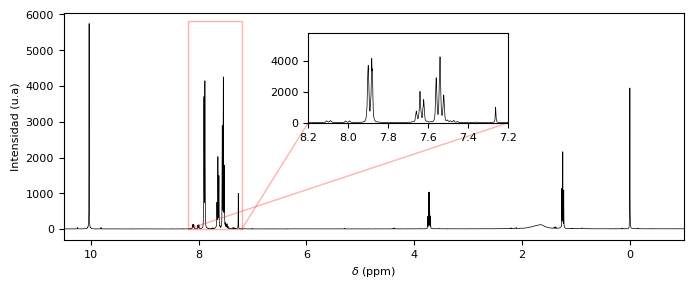
\includegraphics[width=\linewidth]{data/H-Benzaldehido}
	\caption{$^1$H-NMR del benzaldeh\'ido usado en la s\'intesis.}
	\label{fig: HNMR-Benzaldehido}
\end{figure}
\begin{figure}[h]
	\centering
	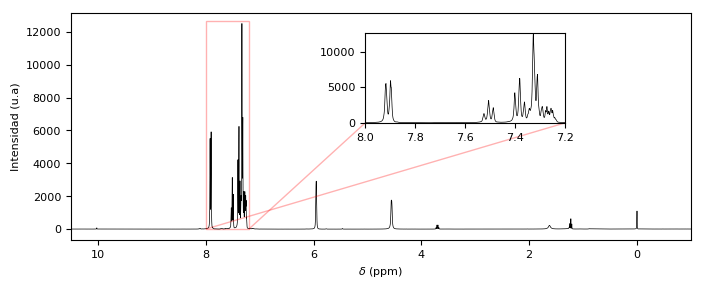
\includegraphics[width=\linewidth]{data/H-Benzoina}
	\caption{$^1$H-NMR de la benzo\'ina.}
	\label{fig: HNMR-Benzoina}
\end{figure}
\begin{figure}[h]
	\centering
	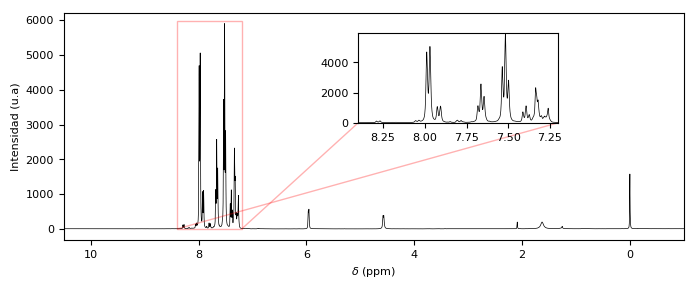
\includegraphics[width=\linewidth]{data/H-BenzilCu}
	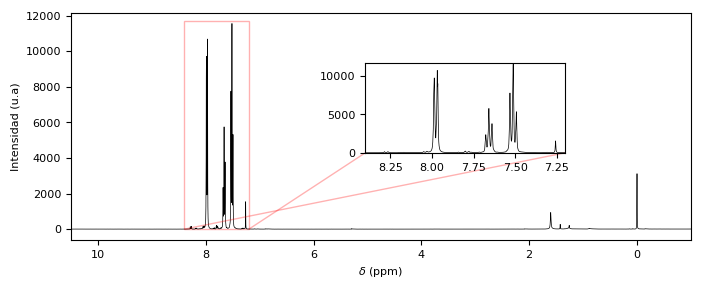
\includegraphics[width=\linewidth]{data/H-BenzilHNO3}
	\caption{$^1$H-NMR del benzil para los dos m\'etodos de s\'intesis. En la posici\'on superior la oxidaci\'on con acetato de cobre, y abajo con \'acido n\'itrico.}
	\label{fig: HNMR-Benzil}
\end{figure}
\begin{figure}[h]
	\centering
	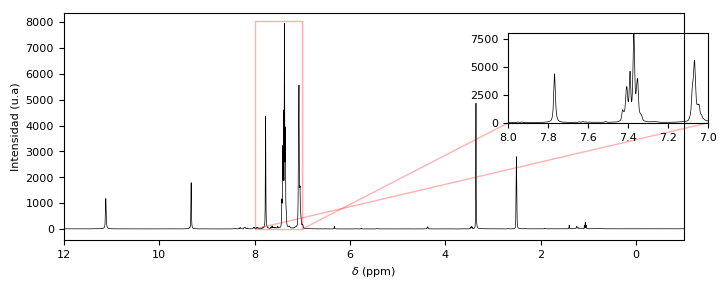
\includegraphics[width=\linewidth]{data/H-Dilatin_So}
	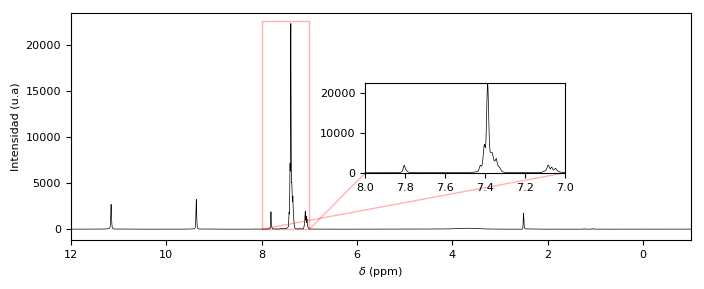
\includegraphics[width=\linewidth]{data/H-Dilatin}
	\caption{$^1$H-NMR del producto final. En la posici\'on superior se muestra el producto obtenido usando ultrasonido, y abajo con reflujo.}
	\label{fig: HNMR-Dilantin}
\end{figure}

\end{document}